% \documentclass[review]{elsarticle}
\documentclass[preprint,12pt]{elsarticle} 
\graphicspath{{images/}}

\usepackage{lineno,hyperref}
\usepackage{algorithm}
\usepackage{algorithmic}
\modulolinenumbers[5]

\journal{Physica A: Statistical Mechanics and its Applications}

\bibliographystyle{elsarticle-num}

\usepackage{mathrsfs}
\usepackage{amsmath}
\usepackage{amssymb}
\usepackage{multirow}
\usepackage{url}



%%%%%%%%%%%%%%%%%%%%%%%
%% Elsevier bibliography styles
%%%%%%%%%%%%%%%%%%%%%%%
%% To change the style, put a % in front of the second line of the current style and
%% remove the % from the second line of the style you would like to use.
%%%%%%%%%%%%%%%%%%%%%%%

%% Numbered
%\bibliographystyle{model1-num-names}

%% Numbered without titles
%\bibliographystyle{model1a-num-names}

%% Harvard
%\bibliographystyle{model2-names.bst}\biboptions{authoryear}

%% Vancouver numbered
%\usepackage{numcompress}\bibliographystyle{model3-num-names}

%% Vancouver name/year
%\usepackage{numcompress}\bibliographystyle{model4-names}\biboptions{authoryear}

%% APA style
%\bibliographystyle{model5-names}\biboptions{authoryear}

%% AMA style
%\usepackage{numcompress}\bibliographystyle{model6-num-names}

%% `Elsevier LaTeX' style
%\bibliographystyle{elsarticle-num}
%%%%%%%%%%%%%%%%%%%%%%%
\def\l{\left\langle}
\def\r{\right\rangle}
\usepackage{mathrsfs}
\usepackage{amsmath}
\usepackage{amssymb}%

\begin{document}
	
	\begin{frontmatter}
		
		
		\title{Low-temperature states of the Ising $\pm J$ model on a square lattice}
		
		\author[FEFU,IPM]{V. O. Trukhin\corref{mycorrespondingauthor}}
		\ead{trukhin.vo@dvfu.ru}
		\author[FEFU]{E. I. Prokhorov\corref{mycorrespondingauthor}}
		\ead{prokhorov.ei@dvfu.ru}
		\author[FEFU,IPM]{A. G. Makarov\corref{mycorrespondingauthor}}
		\ead{makarov.ag@dvfu.ru}
		\author[FEFU,IPM]{K. V. Nefedev\corref{mycorrespondingauthor}}
		\ead{nefedev.kv@dvfu.ru}
		\affiliation[FEFU]{organization={Far Eastern Federal University},
		addressline={10 Ajax Bay, Russky Island}, 
		city={Vladivostok},
		postcode={690922}, 
		state={Primorsky Krai},
		country={Russian Federation}}
		\affiliation[IPM]{organization={Institute of Applied Mathematics, Far Eastern Branch, Russian Academy of Science},
		addressline={Radio Street, 7}, 
		city={Vladivostok},
		postcode={690041}, 
		state={Primorsky Krai},
		country={Russian Federation}}
		
		\begin{abstract}
			
			Using the complete enumeration method, we accurately calculated all possible states of the Edwards-Anderson model on a simple square lattice of $8 \times 8$ spins. The ground state energies of the studied finite-size samples were determined. The macroscopic degeneracy of the ground state in frustrated spin systems arises from the combinatorics of frustrated plaquettes, i.e., the number of ways to place frustrated spin pairs on the lattice. The algorithm for calculating energy, spin excess, and ground state configurations is based on identifying the arrangement of frustrations. The dependence of the ground state spin excess in the Edwards-Anderson model on an external magnetic field has a discrete (step-like, stair-like) character. Critical values of the external magnetic field, at which large peaks in residual entropy occur, were calculated. The nature of these large entropy peaks is explained by the fact that, at certain critical values of the external magnetic field, the sum of several spin configurations with different interaction energies and Zeeman energies, i.e., with different values of spin excess, will have the same total energy. The degeneracy multiplicities of states with the same total energy are summed up at the critical magnetic field value. The areas of existence of low-temperature states have been determined.
			
		\end{abstract}
		
		\begin{graphicalabstract}
		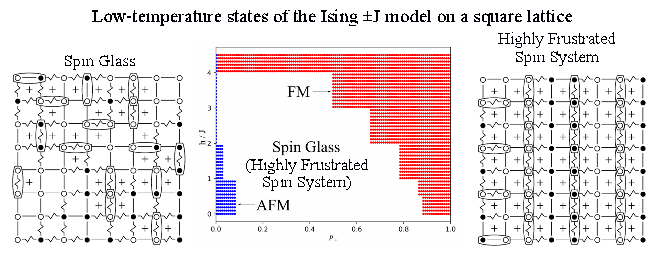
\includegraphics[width=1.2\linewidth]{Graphical Abstract.pdf}
		\end{graphicalabstract}
		
		
		\begin{highlights}
			\item The properties of frustrated bonds in ground state configurations of the $\pm J$ Ising model on a square lattice have been determined.  
			\item Peaks in entropy and magnetization in the field for the ground state have been established.  
			\item The areas of existence of ground states have been determined.  
			\item The phase diagram at zero temperature in an external magnetic field has been constructed.
		\end{highlights}  
		
		
		\begin{keyword}
			Ising model, Ground state, GPU and CPU high performance calculations, statistical physics.
		\end{keyword}
		
	\end{frontmatter}
	
	\linenumbers
	
	%\newpage
	\tableofcontents
	
	\newpage
	\section{Introduction}
	
	Models of frustrated systems are among the most important research topics in statistical mechanics. Ising spin glass in the Edwards-Anderson (EA) model is one of the simplest spin glass model with short-range interactions \cite{edwards1975theory}. Despite its seeming simplicity, the low-temperature properties of this model, even in 2D and especially in higher dimensions, remain poorly understood \cite{pal1996ground, hartmann2011ground, newman2022ground}. Spin lattice models with competing ferromagnetic and antiferromagnetic interactions have been studied for many years \cite{binder1986spin, mezard1987spin, lebrecht2004plaquette, valdes2012j, lebrecht2015j, fan2023searching}.
	
	Despite many years of intensive research, the nature of the low-temperature phase of the Ising model for frustrated spin systems with a restricted interaction range remains unsolved \cite{roma2010ground, newman2023proof}. Two of the most important questions concern the properties of the ground state of spin glasses (i.e., at zero temperature), particularly the degeneracy of the ground state and the nature of low-energy excitations \cite{newman2022ground}.
	
	The calculation of the energy, entropy, and spin excess of the ground state of a spin glass with a given Hamiltonian, even without an external magnetic field, is a complex optimization problem. In three dimensions, this problem is NP-hard \cite{barahona1982computational, hartmann2002optimization}. This means that no known algorithm can solve the problem of calculating spin excess, energy, and ground state degeneracy in time proportional to a polynomial function of the linear system size. It is widely believed that no such algorithm can be developed. Currently, no known algorithm combines high accuracy with efficiency \cite{fan2023searching}.
		
	The properties of spin glasses at zero temperature are typically studied using approximate methods \cite{roma2009ground, perez2012ground}. Over time, various approximate approaches for solving spin system models have been developed, but the problem remains relevant due to the lack of an exact solution \cite{rybin2022hybrid, makarova2023canonical, farias2024differentiable, jabar2024magnetic}. However, for some lattices, such as the triangular lattice, it is possible to obtain information about entropy and magnetic properties \cite{jurvcivsinova2024classical}.
	
	Energy of interactions can be computed using optimization methods \cite{hartmann2002optimization, hartmann2004new}, genetic algorithms \cite{holland1992adaptation}, annealing algorithms \cite{kirkpatrick1983optimization}, multicanonical sampling methods \cite{berg1994ground, shevchenko2017multicanonical}, multi-spin cluster methods \cite{makarova2023canonical}, or parallel tempering \cite{PhysRevB.50.16444, roma2009ground}.
	
	Entropy, or the degeneracy of the ground state, is crucial information not only for understanding the low-temperature behavior of spin glasses (or highly frustrated spin systems) but also for the nature of excitations. Even for the 2D Edwards-Anderson model, computing the ground state is a non-trivial problem. Entropy or the degeneracy multiplicity is an even more challenging task. Methods such as the transfer matrix method \cite{PhysRevB.22.288, cheung1983equilibrium, kolan1982ground}, ballistic search \cite{hartmann2000ground}, thermodynamic integration \cite{kirkpatrick1977frustration, binder1985monte, roma2004ground}, and multicanonical sampling \cite{berg1994ground, shevchenko2017multicanonical} have been developed to address this issue. However, for finite systems with a countable number of spins, approximate methods are unlikely to be applicable.  
	
	Spin system models on lattices provide an ideal platform for exploring complex magnetic ground states with excitations, and their investigation is important for the advancement of physics \cite{lacroix2011introduction}. This research includes calculation of the critical switching fields between ground states in an external magnetic field, entropy peaks during transitions between ground states, and correlation functions \cite{ramirez2004effect, rosas2004random, andriushchenko2019large}.  
	
	Studying the energy landscape of low-energy states in spin glasses~\cite{biswas2023energy} remains an open problem, as does the investigation of highly frustrated spin systems. An intriguing question is identifying the relative fraction (or concentration) of ferromagnetic (or antiferromagnetic) exchange interactions at $T=0$ that results in a transition between ferromagnetism and spin glass states (or between anti-ferromagnetism and spin glass states) \cite{gruzberg2001random, honecker2001universality, picco2006strong, tsomokos2011interplay, zimmer2022role}. The thermodynamic properties and phase diagram of the ground state for molecular clusters with a small number of spins were calculated in \cite{dias2023ground}.
	
	Ground-state configurations, as well as excitations in the ground state and low-energy states of spin glasses, residual entropy at low temperatures, are actively studied in models with long-range dipolar interactions \cite{makarova2021low, singh2024micromagnetic}. The spin glass ground states is both essential for understanding the nature of disordered magnets and many other physical systems and also proves useful for solving a wide range of complex combinatorial optimization problems in various disciplines. Despite decades of effort, no algorithm with both high accuracy and efficiency has yet been developed \cite{fan2023searching}.  
	
	Estimation of the ground state energy and understanding the nature of its macroscopic degeneracy have remained open problems for many years. At low temperatures, the spin glass in its ground state is realized solely through configurations with minimal interaction energy, while the ensemble of other configurations in the Gibbs distribution plays no role. Ground-state energies calculated by various methods in studies \cite{thouless1977solution, sherrington1975solvable, tanaka1980analytic, klein1976comparison, kirkpatrick1978infinite, karandashev2019global, palmer1999ground, campbell2004energy, roma2009ground} show significant variability. It will be shown below that this variability may be related to the distribution of frozen disorder in the bonds, i.e., competing ferromagnetic and antiferromagnetic interactions. For a finite number of spins, the ground state energy strongly depends on the specific realization of the distribution $\left\lbrace J_{ij} \right\rbrace$.  
	
	In this work, we utilized an complete enumeration algorithm \cite{dias2023ground, padalko2021parallel} to solve the problem of ground state energy for a finite number of spins, to calculate the degeneracy of this state, and to determine the distribution of spin excess.
	
	\section{Complete enumeration solution}
	
	To investigate the problem, an complete enumeration algorithm was developed. Energy of $t$-configuration:
	
	\begin{equation}
		E_t = -\sum^{N - 1}_{i=1}\sum^N_{j = i + 1} J_{ij} S_i S_j - h \sum^N_{i=1} S_i.
		\label{eq:ising_energy}
	\end{equation}
	
	We have competing antiferromagnetic ($J_{ij} = -1$) and ferromagnetic ($J_{ij} = +1$) interactions between nearest neighbor spins (Ising spin variables) $S_i = \pm1$, $h$ - external magnetic field in units of $|J_{ij}|$. In the figure captions we will omit the modulus sign for $J_{ij}$.
	
	\begin{equation}
		M_t = \sum^N_{i=1} S_i.
		\label{eq:spin_excess} 
	\end{equation}
	$M$ is a spin excess of given configuration. Each configuration is recognized by two parameters, $E$ and $M$.
	
	
	Alternating nature of exchange integrals $J_{ij}$ may be attributed to distortions in the arrangement of atoms on the lattice or oscillations in electron density.
	
	Let consider a chain of three spins ($L = 3$) interacting ferromagnetically. Hence, all $J_{ij} = +1$. Let $\beta = (kT)^{-1}$, where $k = 1$ -- Boltzmann constant, T -- temperature in units of $|J_{ij}|$. The ground state presented by the configurations at $T \rightarrow 0$. Despite the fact that the ground state is of most interest in this work, we have to search through all $2^N$ states to calculate it accurately. By definition:
	
		\begin{equation}
		Z = \sum_{t = 1}^{2 ^ N} e^{-\beta E_t},
		\label{eq:stat_difinition}
	\end{equation}
	
	\noindent is partition function. Magnetization is defined as: 
	
	\begin{equation}
		\langle M \rangle = \frac{1}{Z} \sum_{t = 1}^{2^N} M_t e^{-\beta E_t}.
		\label{magnetization}
	\end{equation}
	
	Let $Z_3$ be the partition function for a chain of 3 spins with open boundary conditions (all interactions is ferromagnetic $J_{ij} = +1$):
		\begin{equation}
		Z_3 = e^{2\beta + 3h\beta} + 2e^{h\beta} + e^{- 2\beta + h\beta } + e^{- 2\beta -h\beta}  + 2e^{-h\beta} + e^{2\beta - 3h\beta}.
		\label{eq:stat_3}
	\end{equation}

	Now, let us attach a second chain parallel to the first one. Assuming all interactions are ferromagnetic:
	
	\begin{equation}
		\label{eq:stat_z3}
		\begin{alignedat}{2}
			Z_6 =  Z_{3i}Z_{3j}I(Z_{3i},Z_{3j}).
		\end{alignedat}
	\end{equation}

	\noindent where $I(Z_{3i},Z_{3j})$ is the state contribution of the interaction energy between two chains in states $Z_{3i}$ and $Z_{3j}$. For example, if the state of the first chain is $e^{2\beta+3h\beta}$ (all spins ``up'') and the second chain is $e^{2\beta-3h\beta}$ (all spins ``down''), then $I(e^{2\beta+3h\beta}, e^{2\beta-3h\beta})=e^{-3\beta}$. Thus the partition function of two connected chains:
	
		\begin{equation}
			\label{eq:stat_6}
			\begin{alignedat}{3}
			Z_6 = Z_{3}e^{2\beta + 3h\beta}I(Z_{3i}, e^{2\beta + 3h\beta}) + 2Z_{3}e^{h\beta}I(Z_{3i}, e^{h\beta}) + \\
			Z_{3}e^{- 2\beta + h\beta }I(Z_{3i}, e^{- 2\beta + h\beta }) + Z_{3}e^{- 2\beta -h\beta}I(Z_{3i}, e^{- 2\beta -h\beta})  + \\
			2Z_{3}e^{-h\beta}I(Z_{3i}, e^{-h\beta}) + Z_{3}e^{2\beta - 3h\beta}I(Z_{3i}, e^{2\beta - 3h\beta}).
			\end{alignedat}
		\end{equation}
	
	As a result, the partition function for a $3 \times 2$ lattice is:
	\begin{equation}
		\label{eq:stat_6_res}
		\begin{alignedat}{3}
			Z_6 = 4 e^{ - 3 \beta-2 h\beta} + 4 e^{- 3 \beta+2 h\beta} + 5 e^{- \beta-2 h\beta } + 5 e^{- \beta+2 h\beta } + 2 e^{-7 \beta} + 4 e^{-3 \beta} + \\
			8 e^{-\beta} + 6 e^{\beta} + 2 e^{\beta-4 h\beta } + 4 e^{\beta-2 h\beta } + 4 e^{\beta+2 h\beta } + 2 e^{\beta+4 h\beta } + \\
			4 e^{3 \beta-4 h\beta } + 2 e^{3 \beta-2 h\beta } + 2 e^{3 \beta+2 h\beta } + 4 e^{3 \beta+4 h\beta } + e^{7 \beta-6 h\beta } + e^{7 \beta+6 h\beta }.
		\end{alignedat}
	\end{equation}
Then add one more chain in the same way and calculate the partition function for a $3 \times 3$ lattice:
\begin{equation}
	\label{eq:stat_9_un}
	\begin{alignedat}{2}
		Z_9 =  Z_{3}Z_{6}I(Z_{3i},Z_{6j}).
	\end{alignedat}
\end{equation}
Equations \eqref{eq:stat_z3}, \eqref{eq:stat_6}, \eqref{eq:stat_6_res} and  \eqref{eq:stat_9_un} show a scheme for calculating the statistical sum by connecting one-dimensional chains into a two-dimensional lattice. Algorithm \ref{alg:addititional_algorithm} \cite{trukhin2024glaurung} works on this principle, but operates on energies, spin excesses and degeneracy of states. Temperature is not used in this complete enumeration.
	
	Note that when connecting the chains to each other, it is necessary to devise a multiplication operator that will multiply the terms of the partition function by the interaction energies of spins located in different chains. This is difficult to accomplish even for open boundary conditions. Therefore, instead of searching for an exact analytical solution, the authors developed the complete enumeration algorithm.
	
	
	\begin{algorithm}[H]
		\textbf{INPUT:} Lattice size and geometry (number and coordinates of spins, boundary conditions, number of neighbors), distribution of exchange constants.\\
		\textbf{OUTPUT:} Partition function parameters, density of states (degeneracy, energy and spin excess).
		\begin{algorithmic}
			\STATE {Compute state density for the first 1D chain.}
			\FOR {Number of lattice layers \\}
			{
				\STATE {Compute state density for the attached 1D chain.}
				\FOR {Length of the 1D chain \\}
				{
					\STATE {Compute state density for the resulting lattice.}
				}
				\ENDFOR \\
			}
			\ENDFOR
		\end{algorithmic}
		\caption{Computing partition function parameters by attaching chains.}
		\label{alg:addititional_algorithm}
	\end{algorithm}
	
	A two-dimensional lattice is assembled from $L$ elements (one-dimensional chains with size $L$). The enumeration in Algorithm \ref{alg:addititional_algorithm} is performed only once for each element to be joined. As a result, for a square lattice of size $L \times L = N$, the computational complexity of complete enumeration is reduced from $2^{N}$ to $L \times 2^L + (L - 1) \times 2^L$. Thus, the performance gain is approximately 92\% for a 9-spin lattice and spans 27 orders of magnitude for a 100 spins. The gain in processing speed arises due to the exclusion of the operation of storing information about the states of the already processed part of the lattice. This leads to the impossibility of processing the lattice with periodic boundary conditions. The analysis of dimensional effects at scaling was carried out in paper \cite{trukhin2024thermodynamic} and showed that the influence of surface spins on the obtained results is insignificant. Thus, the obtained results are relevant for a regular lattice.
	
	\section{Plaquette combinatorics}
	
	Let by a plaquette we mean a closed chain of spins of minimal length \cite{lebrecht2015j}. In the following examples on a square lattice, the plaquettes are elementary squares, see Figures \ref{fig:Type1}, \ref{fig:Type2}, and \ref{fig:Type3}. In the Edwards-Anderson spin glass model, the plaquettes can be classified into three possible types. 
	
	If $P_+$ is the relative amount of ferromagnetic ($J_{ij}=+1$) exchange integrals, then Type-I, see Figure \ref{fig:Type1}, belongs to the plaquettes in which $P_+=0.5$. For Type-II, $P_+=0.75$ or $P_+=0.25$ (Figure \ref{fig:Type2}). For Type-III, $P_+=1.0$ or $P_+=0.0$ (Figure \ref{fig:Type3}). Straight and jagged lines in the figures correspond to ferromagnetic and antiferromagnetic bonds, respectively. White and black circles in the figures correspond to ``up'' and ``down'' spins in one of the ground state configurations. Frustrated pairs of spins are circled. By a frustrated spin pair (frustated bond) we mean a pair (bond) for which the interaction energy is positive. Thus frustration is the excitation with a given localization, coordinates in ground state configuration.
	
	
	\begin{figure}[H]
		\centering
		\begin{minipage}[t]{0.3\textwidth}
			\centering
			\resizebox{45px}{45px}{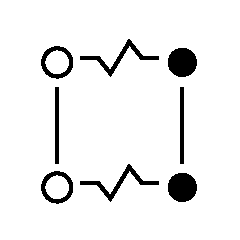
\includegraphics{pictures/Type1_1.eps}}
			\hspace{-4pt} 
			\resizebox{45px}{45px}{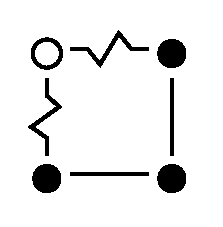
\includegraphics{pictures/Type1_2.eps}}
			\caption{Systems consisting of Type-I plaquette ($P_+=0.5$).}
			\label{fig:Type1} 
		\end{minipage}
		\hspace{5pt} 
		\begin{minipage}[t]{0.3\textwidth}
			\centering
			\resizebox{45px}{45px}{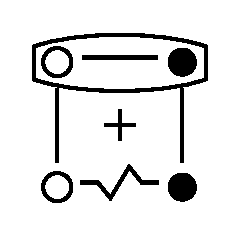
\includegraphics{pictures/Type2_1.eps}}
			\hspace{-2pt} 
			\resizebox{45px}{45px}{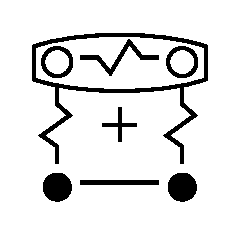
\includegraphics{pictures/Type2_2.eps}}
			\caption{Systems consisting of Type-II plaquette ($P_+=0.75, P_+=0.25$). Frustrated pairs of spins are circled.}
			\label{fig:Type2}
		\end{minipage}
		\hspace{5pt}
		\begin{minipage}[t]{0.3\textwidth}
			\centering
			\resizebox{45px}{45px}{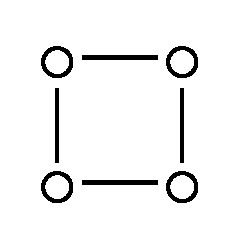
\includegraphics{pictures/Type3_1.eps}}
			\hspace{-4pt} 
			\resizebox{45px}{45px}{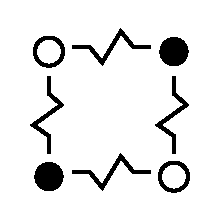
\includegraphics{pictures/Type3_2.eps}}
			\caption{Systems consisting of Type-III plaquette ($P_+=1.0, P_+=0.0$).}
			\label{fig:Type3}
		\end{minipage}
	\end{figure}
	
	
	There are $2^N$ configurations for each these and next considered plaquettes.
	It was found that frustration (excitation or positive energy of the exchange interaction in $ij$-pair of spins) in the ground state necessarily appears in Type-II plaquettes, which are marked by the ``$+$'' sign. The frustrated pair in Type-II plaquettes can be any pair of spins, Figure \ref{fig:Type2}. Thus, competing ferromagnetic and antiferromagnetic interactions between nearest neighbors lead to the presence of at least one frustration in the ground state configurations only if a Type-II plaquette is formed.
	
	Hereinafter we understand the system as a set of N interacting elements (moments, spins, plaquettes etc.). If the system consists of two Type-II plaquettes, for example, as shown in Figure \ref{fig:Type2_32}, the frustrated pair is necessarily located at the intersection of the plaquettes. This minimizes the energy, regardless of the distribution of exchange interactions in the rest of the lattice. This arrangement of frustration satisfies the rule: each Type-II plaquette necessarily has at least one frustration.
	
	\begin{figure}[H]
		\centering
		\begin{minipage}{0.2\textwidth}
			\centering
			(a)
			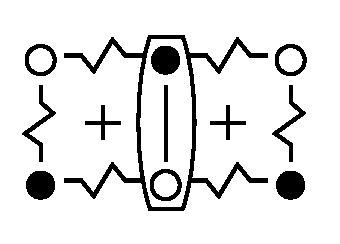
\includegraphics[width=1\textwidth]{pictures/Type2_3x2.eps}
			\label{fig:Type2_3x2}
		\end{minipage}
		\hspace{20pt}
		\begin{minipage}{0.2\textwidth}
			\centering
			(b)
			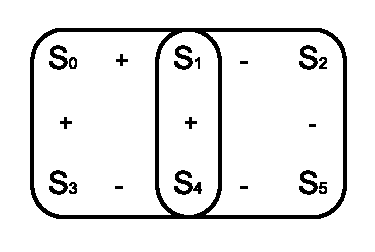
\includegraphics[width=1\textwidth]{pictures/Type2_3x2_2.eps}
			\label{fig:Type2_3x2_2}
		\end{minipage}
		\caption{The ground state configurations of the systems consisting of two Type-II plaquettes with $P_+\approx0.14$ (a) and $P_+\approx0.43$ (b).}
		\label{fig:Type2_32}
	\end{figure}
	
	
	It is easy to find the energy, spin excess and configurations of the ground state at the known arrangement of frustrated pairs of spins. The energy of the ground state for the systems, in Figure \ref{fig:Type2_32}(a) and \ref{fig:Type2_32}(b) $E_{gs}/N=(-6+1)/6\approx-0.83$. In the system the energies of 6 pairs are negative and 1 pair is excited (frustrated). Degeneracy $g_{gs}=2$, because ground state configurations have the same energy when flipping each $S_i \rightarrow -S_i$. The ground state spin excess $M_{gs}/N=0$ for the system in Figure \ref{fig:Type2_32}(a) and $M_{gs}/N\approx\pm 0.33$ in Figure \ref{fig:Type2_32}(b).
	In Figures \ref{fig:4x4.1}, there is a Type-II plaquette containing frustration in the center of the lattice. Placing frustration in a non-Type-II plaquette results in another excitation in it. In this example, there are 8 ground state configurations with $E_{gs}/N=-1.25$. Spin excesses are $M_{gs}/N=\pm 0.375$ - Figures \ref{fig:4x4.1}(a) and \ref{fig:4x4.1}(b), $M_{gs}/N=\pm 0.125$ - Figure \ref{fig:4x4.1}(c), $M_{gs}/N=\pm 0.625$ - Figure \ref{fig:4x4.1}(d).
	
	\begin{figure}[H]
		\begin{minipage}[h]{0.2\linewidth}
			\centering(a)
			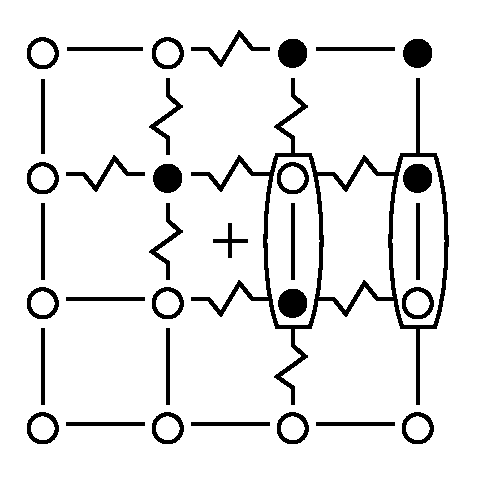
\includegraphics[width=1\linewidth]{pictures/Cl1_Type2_gs1.eps}
		\end{minipage}
		\hfill
		\begin{minipage}[h]{0.2\linewidth}
			\centering(b)
			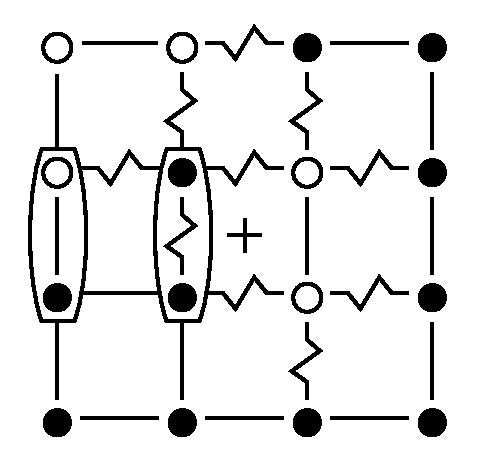
\includegraphics[width=1\linewidth]{pictures/Cl1_Type2_gs2.eps}
		\end{minipage}
		\hfill
		\begin{minipage}[h]{0.2\linewidth}
			\centering(c)
			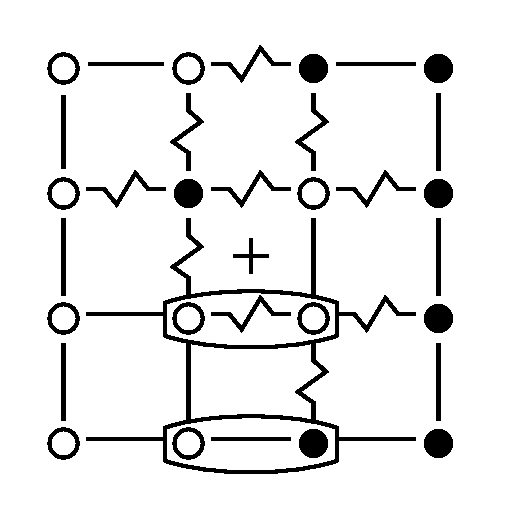
\includegraphics[width=1\linewidth]{pictures/Cl1_Type2_gs3.eps}
		\end{minipage}
		\hfill
		\begin{minipage}[h]{0.2\linewidth}
			\centering(d)
			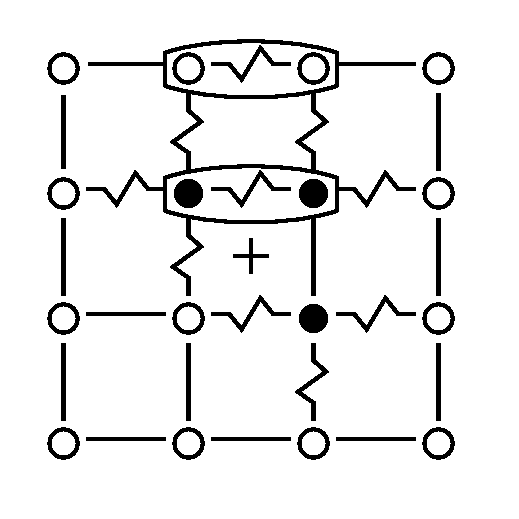
\includegraphics[width=1\linewidth]{pictures/Cl1_Type2_gs4.eps}
		\end{minipage}
		\caption{The ground state configurations of the system $N=16$ spins and a single Type-II plaquette in the middle of the lattice ($P_+\approx0.58$).}
		\label{fig:4x4.1}
		
	\end{figure}
	
	As seen in Figure \ref{fig:4x4.1}(a), two ferromagnetic bonds are frustrated. However, in Figures \ref{fig:4x4.1}(b) and \ref{fig:4x4.1}(c), different bonds become frustrated -- one antiferromagnetic and one ferromagnetic. In Figure \ref{fig:4x4.1}(d), two frustrated antiferromagnetic bonds are also observed. Thus, the absence of localization or a fixed geometric arrangement of frustrated bonds leads to the ground state degeneracy.
	
	For the example in Figure \ref{fig:4x7}, $E_{gs}/N \approx -1.39$, $M_{gs}/N=0$, there are only two ground states $g_{gs}=2$. At the same time, there are three frustrated pairs. Thus, the presence of frustrations in configurations of the ground state does not always lead to macroscopic degeneracy. 
	
	\begin{figure}[H]
		\centering
		\resizebox{150px}{75px}{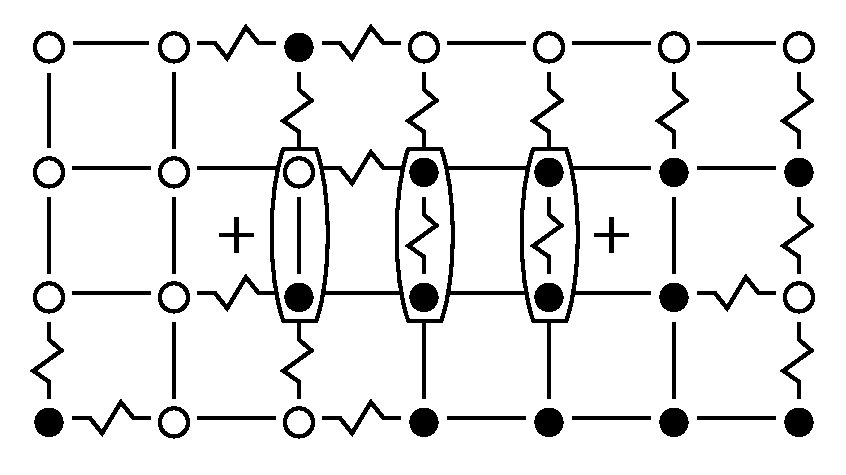
\includegraphics{pictures/Cl7x4_Type2.eps}}
		\caption{The ground state configuration of the system $N=28$ spins and two Type-II plaquettes ($P_+=0.6$).}
		\label{fig:4x7}
	\end{figure}
	
	Figure \ref{fig:5x5.22F} shows an example ($E_{gs}/N=-1.44$, $g_{gs}=4$, $M_{gs}/N=\pm 0.12$ for Figure \ref{fig:5x5.22F}(a) and $M_{gs}=\pm 0.04$ for \ref{fig:5x5.22F}(b)) when two Type-II plaquettes share a common spin. Despite the decrease in the number of frustrated pairs, there is an increase in the ground state degeneracy compared to the previous example. The combinatorics arises because there are several options for the placement of frustrated pairs on the lattice.
	
	\begin{figure}[H]
		\centering
		\begin{minipage}[h]{0.25\linewidth}
			\centering(a)
			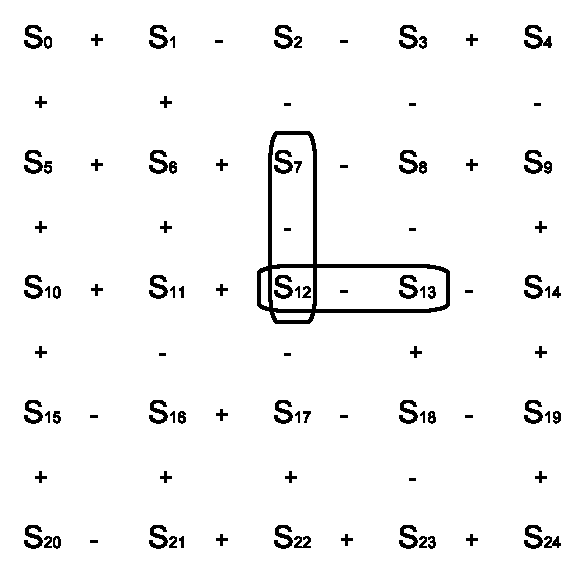
\includegraphics[width=1\linewidth]{pictures/Cl5x5_Type2_gs1.eps}
		\end{minipage}
		\hspace{15pt}
		\begin{minipage}[h]{0.25\linewidth}
			\centering(b)
			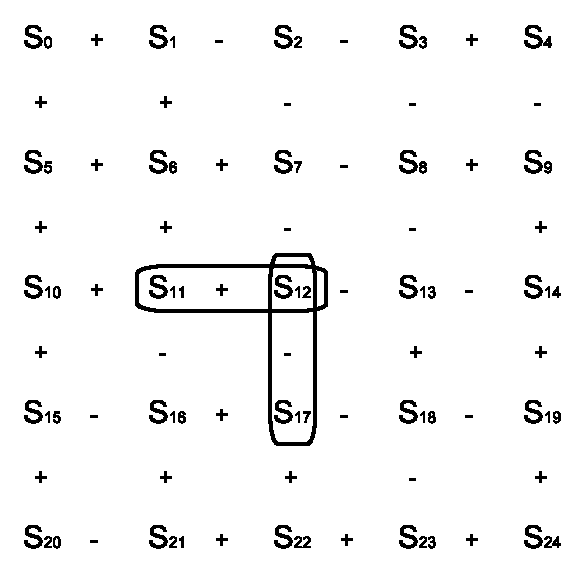
\includegraphics[width=1\linewidth]{pictures/Cl5x5_Type2_gs2.eps}
		\end{minipage}
		\caption{The ground state configurations of the system $N=25$ spins and two Type-II plaquettes ($P_+\approx0.58$).}
		\label{fig:5x5.22F}
	\end{figure}
	
	Thus Type-II plaquettes are the only cause of frustrations in configurations of the ground state. In configuration of the ground state, frustrations are located between Type-II plaquettes or between a plaquette and the edge of the grid, depending on the distances. Macroscopic degeneration of the ground state is due to alternative frustration locations.
	
	\section{Nature of the ground state degeneracy}
	
	It is possible to calculate all ground states by pairwise combination of Type-II plaquettes. Let us consider the operation of the algorithm on the example of a lattice consisting of 64 spins (Figure \ref{fig:12PS_cell64_J72_5}(a)).
	
	\begin{figure}[H]
		\centering
		\begin{minipage}[h]{0.3\linewidth}
			\centering(a)
			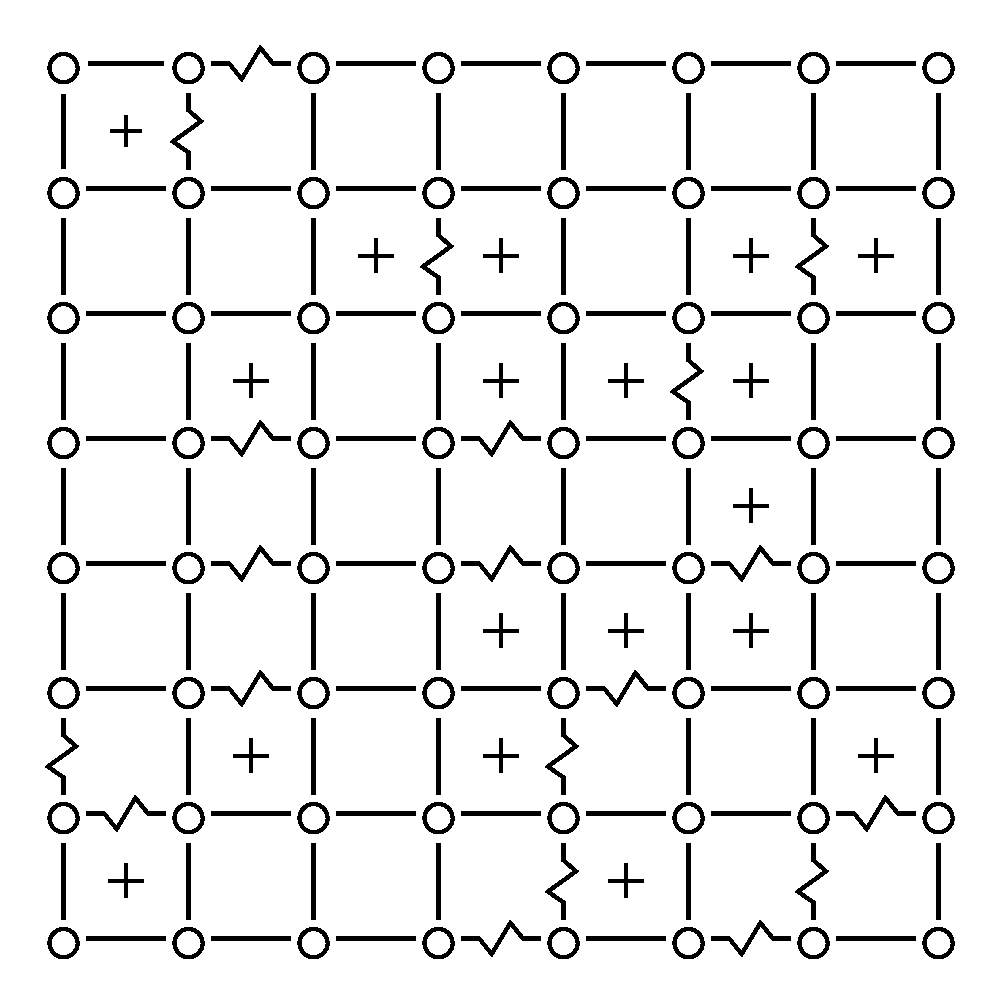
\includegraphics[width=1\linewidth]{pictures/cell64_J72_5.eps}
		\end{minipage}
		\hspace{10pt}
		\begin{minipage}[h]{0.3\linewidth}
			\centering(b)
			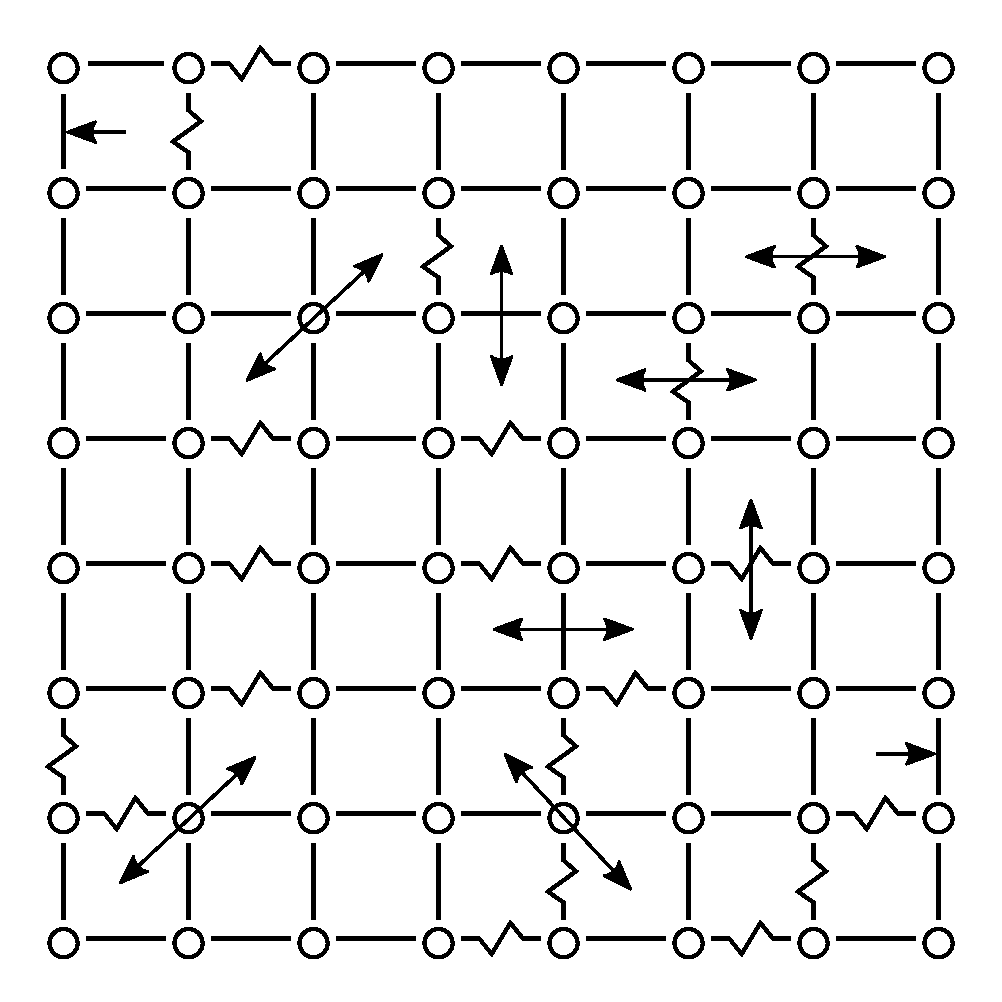
\includegraphics[width=1\linewidth]{pictures/1PS_cell64_J72_5.eps}
		\end{minipage}
		\hspace{10pt}
		\begin{minipage}[h]{0.3\linewidth}
			\centering(c)
			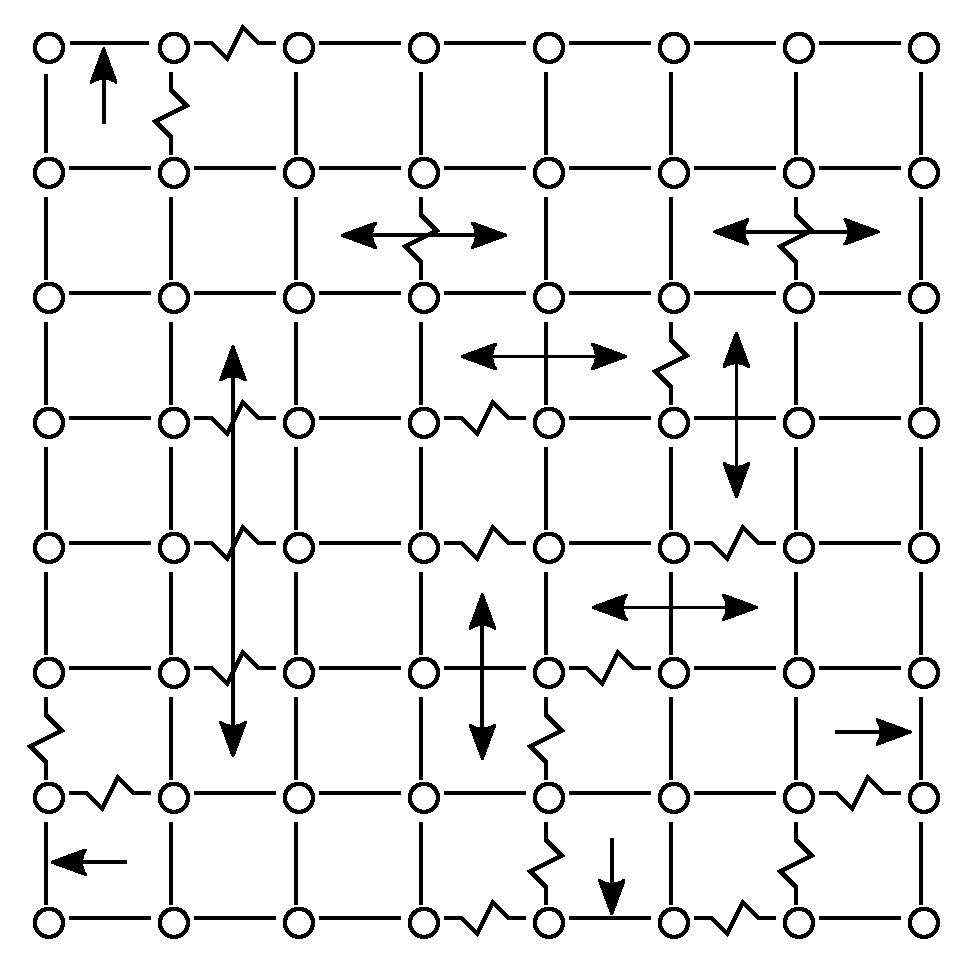
\includegraphics[width=1\linewidth]{pictures/2PS_cell64_J72_5.eps}
		\end{minipage}
		\caption{(a) - An example of a system $N=64$ spins and 18 Type-II plaquettes, (b, c) - combinations of Type-II plaquettes with the minimal number of frustrations ($P_+\approx0.82$).}
		\label{fig:12PS_cell64_J72_5}
	\end{figure}
	
	
	First, each plaquette is assigned coordinates $x$ and $y$. Next, the partitioning of the Type-II plaquettes into pairs is combined. We consider the cases when frustrations occur between each pair of plaquettes and when the placement of excitations occurs between a plaquette and the edge of the lattice. The quantity of frustrations between $i,j$-th pair of plaquettes is defined as $R_{ij} = \left|x_i-x_j\right|+\left|y_i-y_j\right|$.
	
	The quantity of frustrations occurring from the Type-II plaquette to the nearest edge of the lattice is defined as $R_{ij}+1$. Here $i$ is the number of the Type-II plaquette, $j$ is the number of the nearest plaquette on the edge of the lattice. The combinations that have the minimum quantity of frustrations are considered after enumerating all pairs of Type-II plaquettes. Two of them are shown in Figures \ref{fig:12PS_cell64_J72_5}(b) and \ref{fig:12PS_cell64_J72_5}(c).
	
	Based on the combinations obtained, the spin pairs between the plaquettes are marked as frustrated (Figure \ref{fig:12F_cell64_J72_5}).
	
	\begin{figure}[H]
		\centering
		\begin{minipage}[h]{0.3\linewidth}
			\centering(a)
			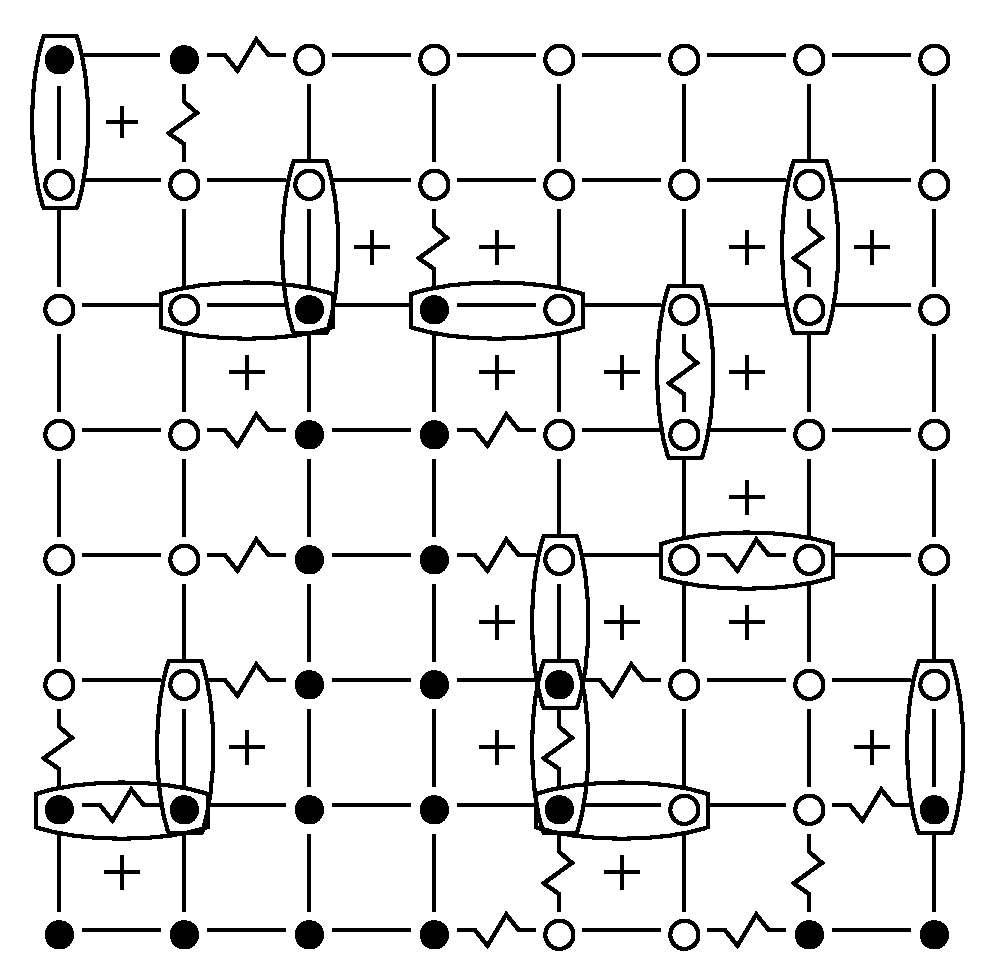
\includegraphics[width=1\linewidth]{pictures/1Conf_cell64_J72_5.eps}
		\end{minipage}
		\hspace{15pt}
		\begin{minipage}[h]{0.3\linewidth}
			\centering(b)
			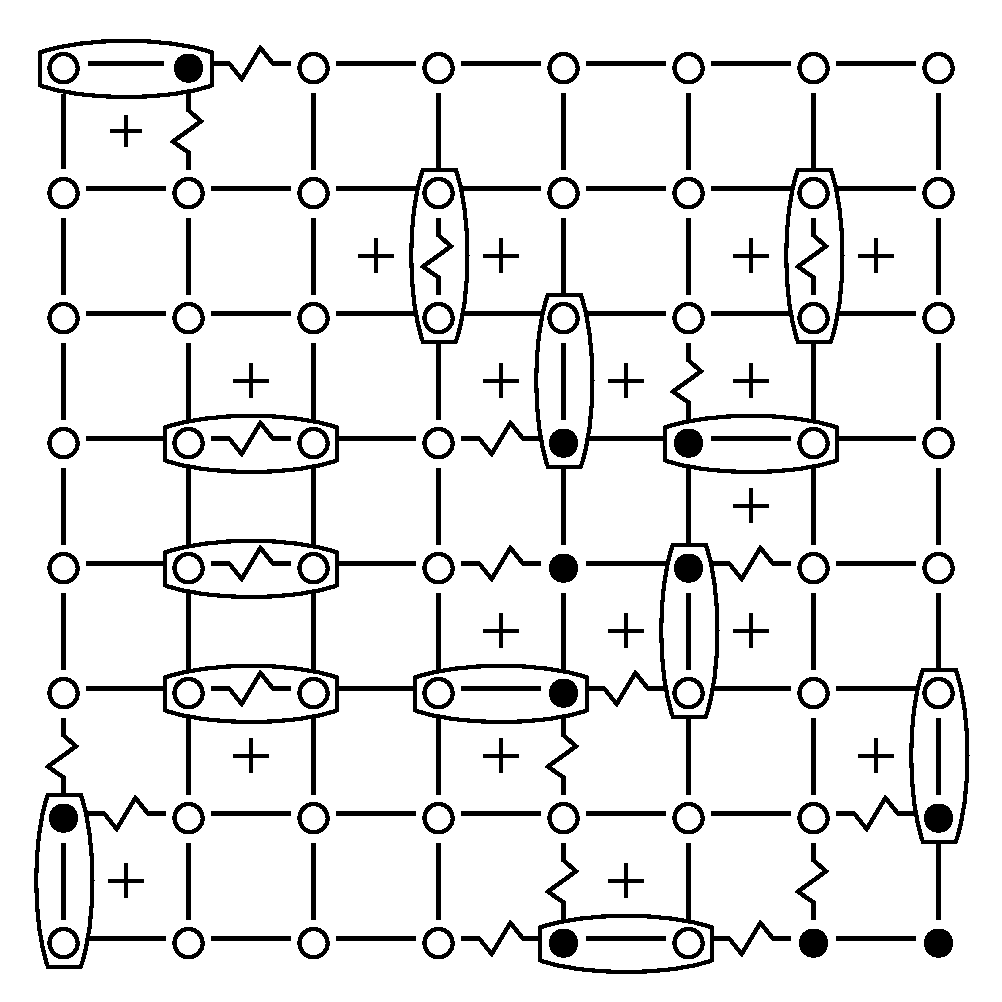
\includegraphics[width=1\linewidth]{pictures/2Conf_cell64_J72_5.eps}
		\end{minipage}
		\caption{Ground state configurations  and plaquettes distribution of the system from Figure \ref{fig:12PS_cell64_J72_5}(a) ($P_+\approx0.82$) correspond to combinations of the Type-II plaquettes \ref{fig:12PS_cell64_J72_5}(b) and \ref{fig:12PS_cell64_J72_5}(c).}
		\label{fig:12F_cell64_J72_5}
	\end{figure}
	
	Figure \ref{fig:g_Mgs} shows information on the distribution of spin excess over the ground state configurations. The distribution $J_{ij}$ is shown in Figure \ref{fig:12PS_cell64_J72_5}. The values $M=0$ and $M=1.0$ are absent for such a distribution $J_{ij}$, $P_+\approx0.82$. This distribution of $J_{ij}$ corresponds to a spin glass, as there are no configurations with a spin excess of $\pm1.0$.
	
	\begin{figure}[H]
		\centering
		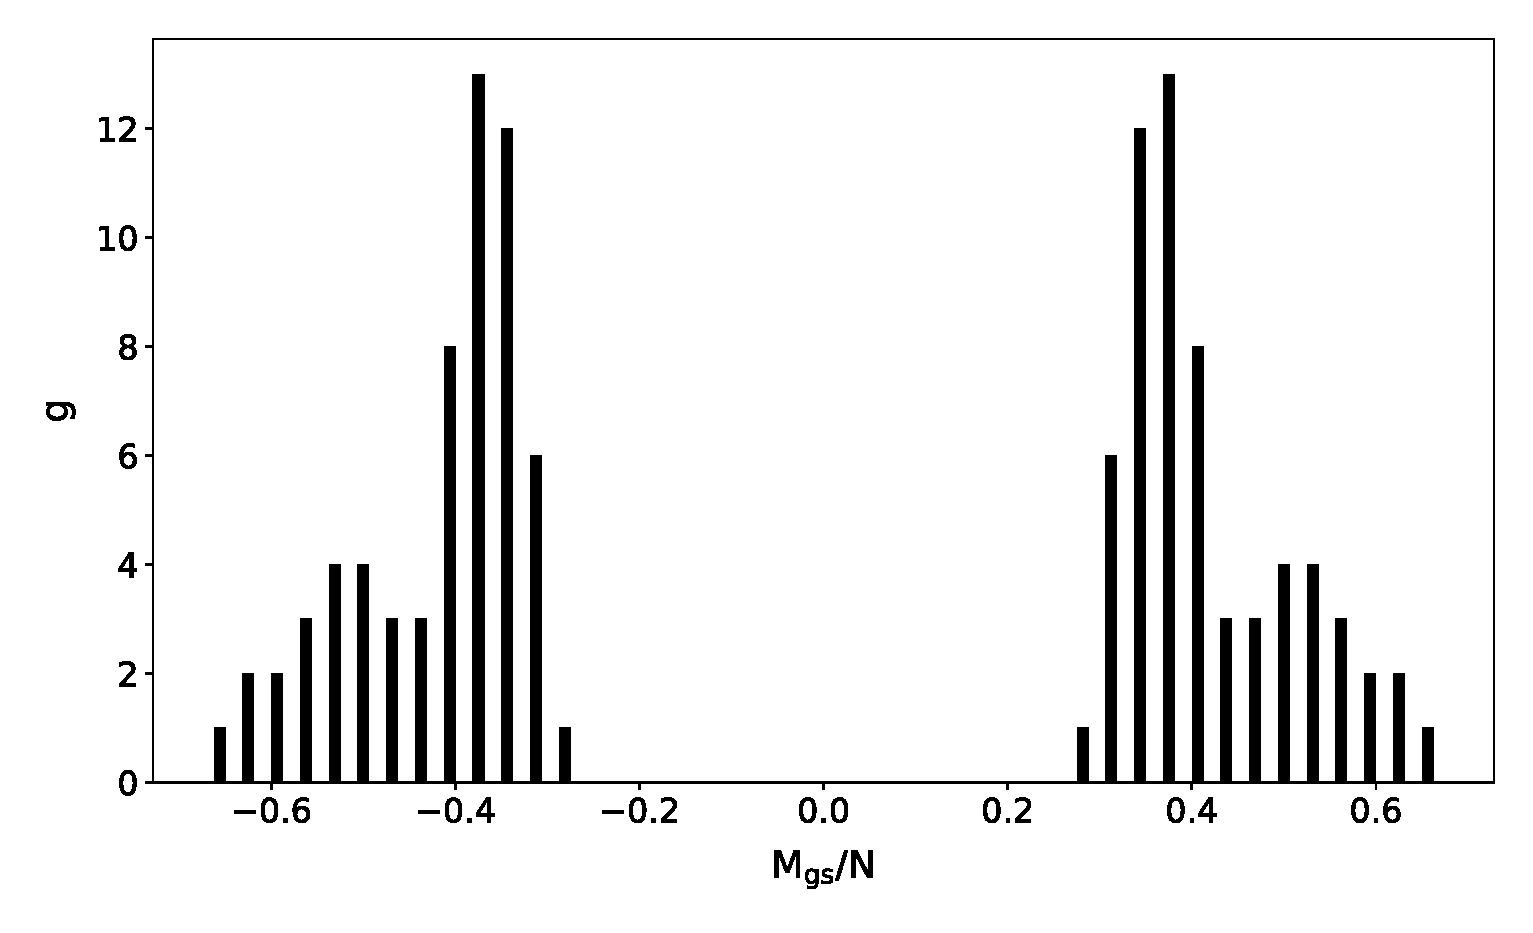
\includegraphics[width=0.8\linewidth]{pictures/g_Mgs.eps}
		\caption{The degeneracy of the ground state for the lattice by Figure \ref{fig:12PS_cell64_J72_5}, $P_+\approx0.82$.}
		\label{fig:g_Mgs}
	\end{figure}
	
	In total, $g_{gs}=124$ configurations of ground state with energy $E_{gs}/N \approx -1.34$ and spin excess $M_{gs}/N$ from $\approx \pm 0.28$ to $\approx \pm 0.66$ were obtained for this lattice. 
	
	Thus, the macroscopic degeneration of the ground state is due to several reasons:
	
	\begin{enumerate}
		\item Different combinations of Type-II plaquettes can produce the same quantity of frustrations, as shown in the previous example in Figures \ref{fig:12PS_cell64_J72_5}(b) and \ref{fig:12PS_cell64_J72_5}(c).
		\item There may be several variants for placing frustrations between plaquettes if the coordinates of these plaquettes are different (Figure \ref{fig:5x5.22F}).
		\item Free boundary conditions can affect degeneracy. For example, in the case of placing a frustrated plaquette next to two boundaries of lattice leads to an increase in the number of options for the placement of frustrations (Figure \ref{fig:4x4.1}).
	\end{enumerate}
	
	\section{Ground state energy}
	
	Calculated the ground state energies of spin glass in the Edwards-Anderson model are presented in Table \ref{tab:Egs}. The table shows that the ground state energy values exhibit significant dispersion.
	
	\begin{table}[h]
		\begin{tabular}{|l|c|c|l|}
			\hline
			Method     &     Distribution $J_{ij}$                         &
			$E_{gs}$                                       &  Ref.                                          \\ \hline
			Thouless-Anderson-Palmer (TAP)& Gaussian &  0                                              & \cite{thouless1977solution}    \\ \hline
			Replica Method   & Gaussian                         & $-2/\pi$                                       & \cite{sherrington1975solvable} \\ \hline
			Partition function   &   -                 & -0.5                                           & \cite{tanaka1980analytic}      \\ \hline
			Mean random field  &   Gaussian  &                   $-1/\sqrt{2\pi}$                               & \cite{klein1976comparison}     \\ \hline
			Monte-Carlo      &   Gaussian    &        -0.76                                          & \cite{kirkpatrick1978infinite} \\ \hline
			Algorithm of Shraudorphs-Kamensky   &  Uniform &     -1.33                                          & \cite{karandashev2019global}   \\ \hline
			Parallel Tempering &   -       & -1.40193                                       & \cite{palmer1999ground}        \\ \hline
			Branch-and-Cut Algorithm  & Bimodal               & -1.40197                         
			& \cite{campbell2004energy}      \\ \hline
			
			Parallel tempering Monte-Carlo    &  Gaussian         & -1.31479                                       & \cite{roma2009ground}          \\ \hline
			
			
			
		\end{tabular}
		\caption{Ground state specific energy obtained by different methods ($P_+\approx$ 0.5).}
		\label{tab:Egs}
	\end{table}
	
	The Figure \ref{fig:E(Q)} shows the dependence of the ground state specific energy $E_{gs}/N$ on the relative amount of ferromagnetic exchange integrals (Gaussian distribution). The points are marked in different colors depending on the number of Type-II plaquettes ($Q$).
	
	\begin{figure}[H]
		\centering
		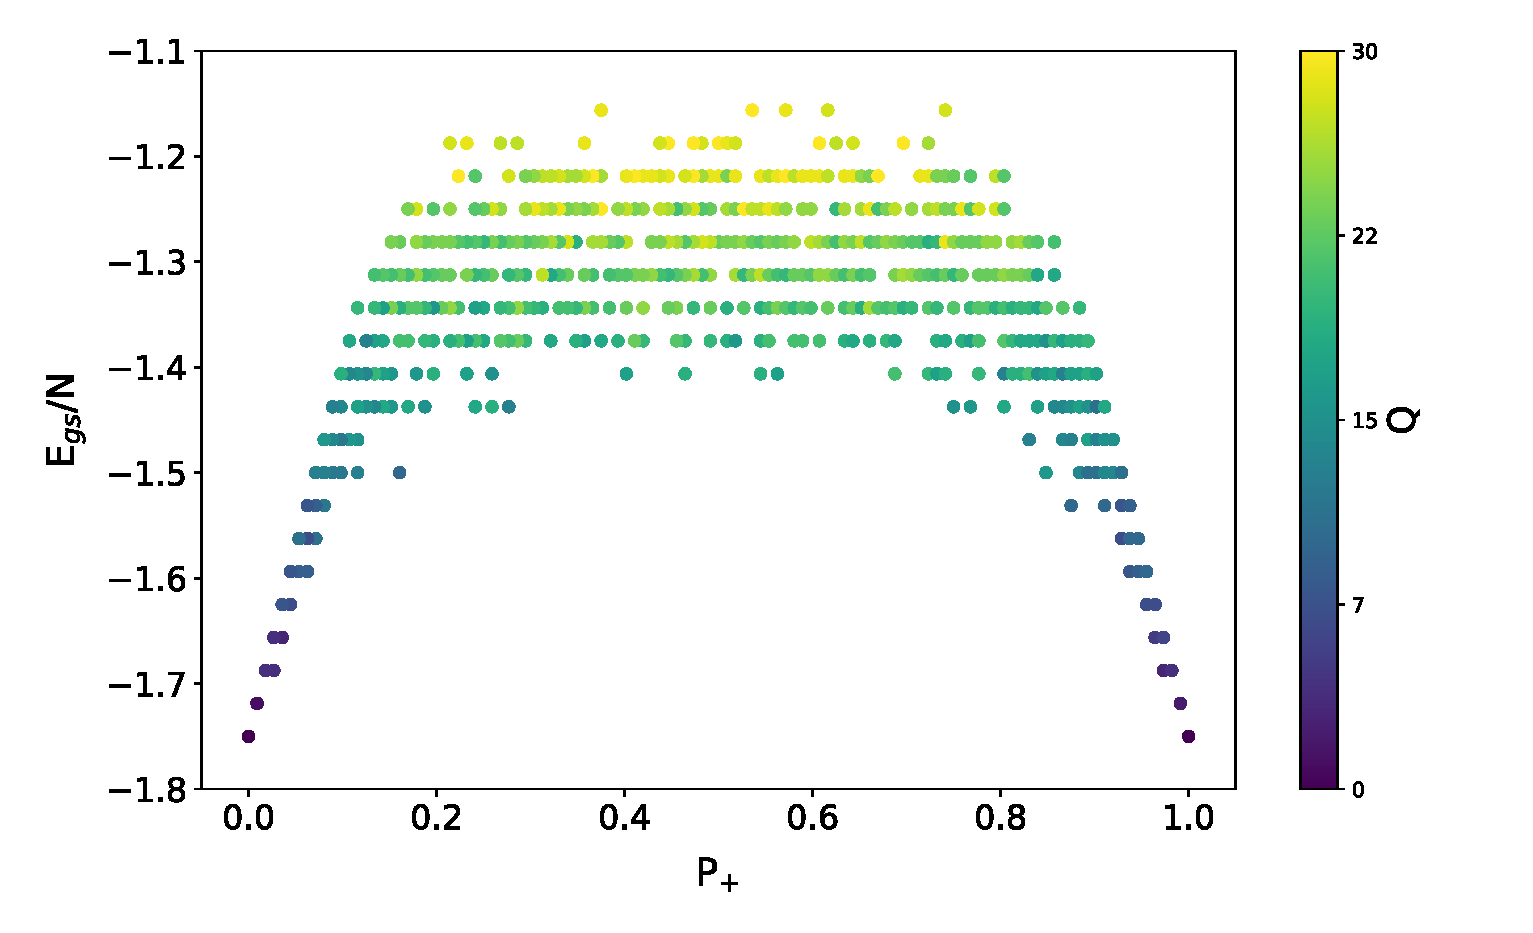
\includegraphics[width=1.0\linewidth]{pictures/E_P_Q.eps}
		\caption{Ground state specific energy as a function of the relative amount of ferromagnetic exchange integrals ($P_+$) for $N=64$. The color scale represents the number of Type-II plaquettes ($Q$) on the lattice.}
		\label{fig:E(Q)}
	\end{figure}
	
	With an increase in the number of Type-II plaquettes $Q$, the ground state energy increases on average. Energy depends not only on the number of Type-II plaquettes but also on their arrangement within the lattice. This explains the dispersion in ground state energy values shown in Figure \ref{fig:E(Q)} and Table \ref{tab:Egs}. An increase in the number of frustrated type II plaquettes leads to an increase in the value of the ground state energy.
	
	
	\begin{figure}[H]
		\centering
		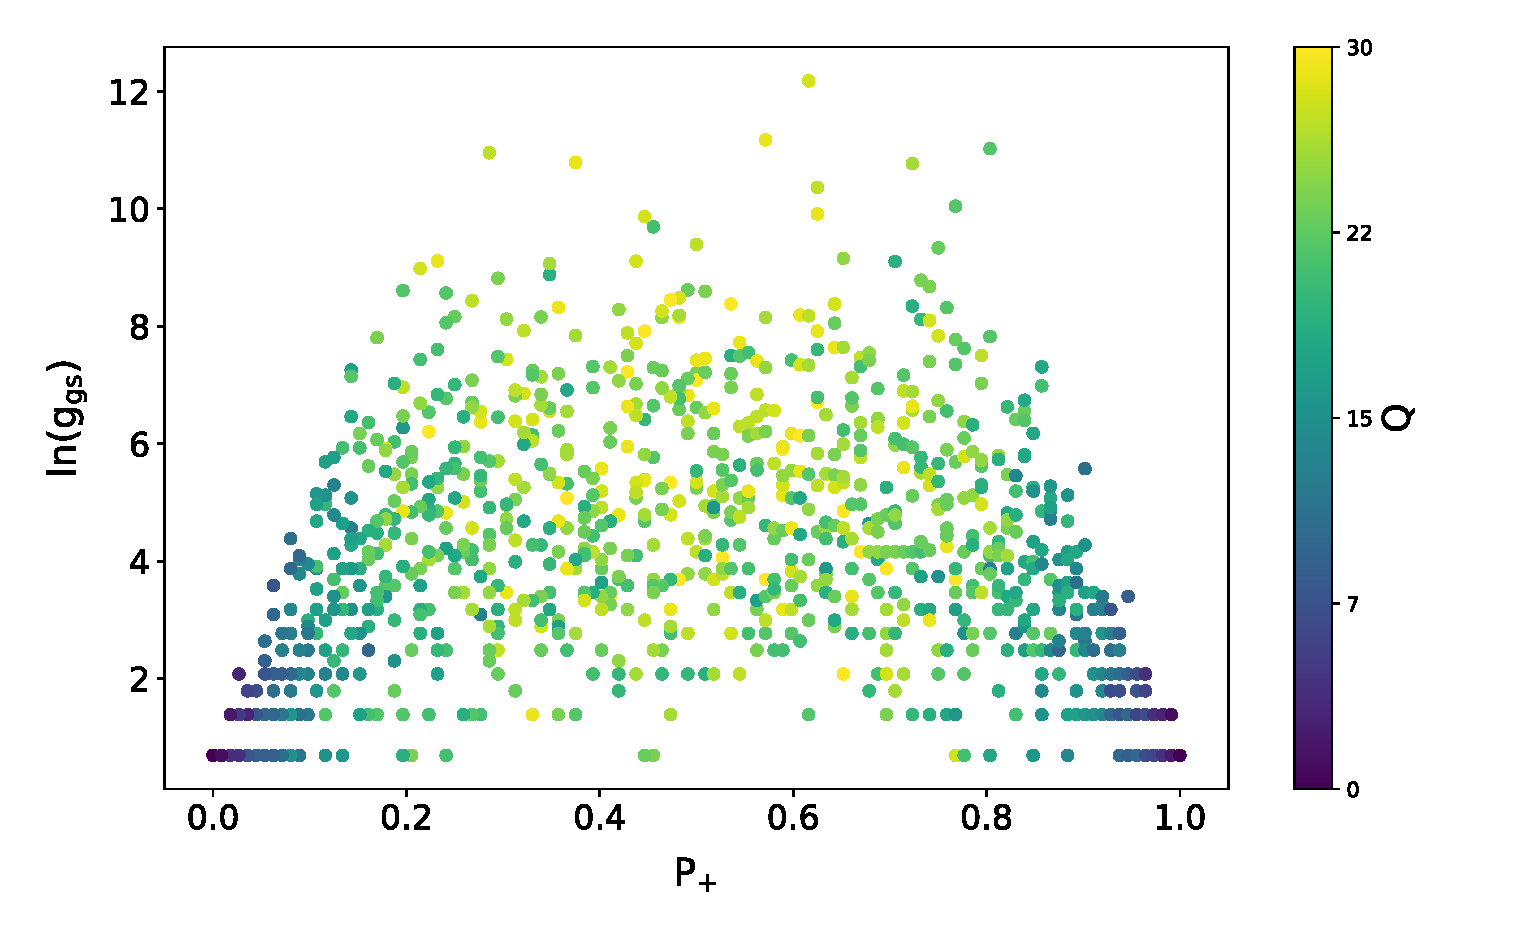
\includegraphics[width=1.0\linewidth]{pictures/lng_P_Q.eps}
		\caption{Ground state degeneracy as a function of the relative amount of ferromagnetic exchange integrals ($P_+$) for $N=64$. The color scale shows the number of Type-II plaquettes ($Q$) in the lattice.}
		\label{fig:g(Q)}
	\end{figure}
	
	The increasing of a number of Type-II plaquettes, and, accordingly, the quantity of frustrations, generally leads to an increase in ground state degeneracy. However, for some samples, an increase in the quantity of frustrations does not result in a growth in ground state degeneracy (see points with the minimum value $g_{gs}=2$ in Figure \ref{fig:g(Q)}). 
	
	\section{Spin models}
	
	Historically, spin ice has been associated with the pyrochlore lattice \cite{skjaervo2020advances, bramwell2020history, udagawa2021spin, ortiz2019colloquium, budrikis2021fifty, castelnovo2012spin}.
	Nowadays, a large number of new spin lattices are emerging. In this paragraph, we aim to clarify the definition of the highly frustrated spin system in the $\pm J$ Ising model.
	
	Let us consider Figure~\ref{fig:cell_SI_SG_64}, which illustrates, for example, three specific cases where the $\pm J$ interactions are arranged in particular patterns.

	\begin{figure}[H]
		\begin{minipage}[h]{0.3\linewidth}
			\centering(a)
			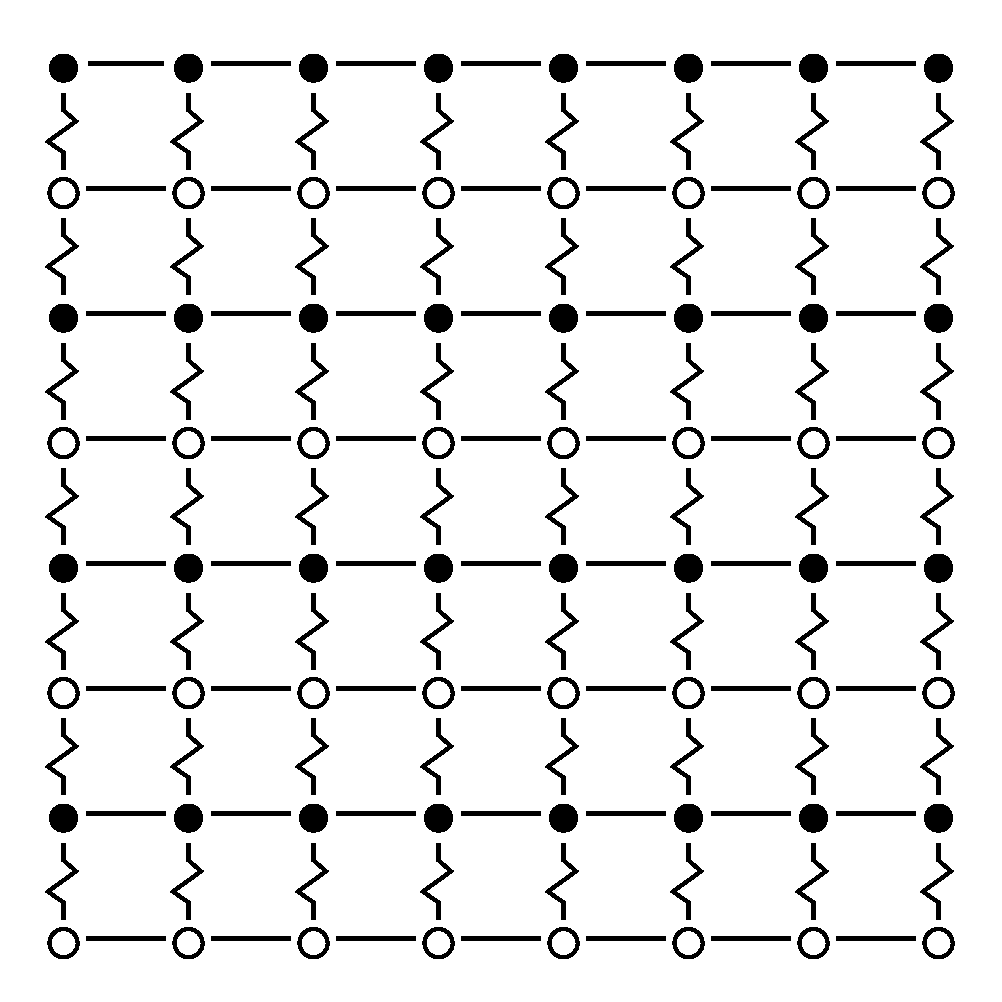
\includegraphics[width=1\linewidth]{pictures/SI_64_J0_1}
		\end{minipage}
		\hfill
		\begin{minipage}[h]{0.3\linewidth}
			\centering(b)
			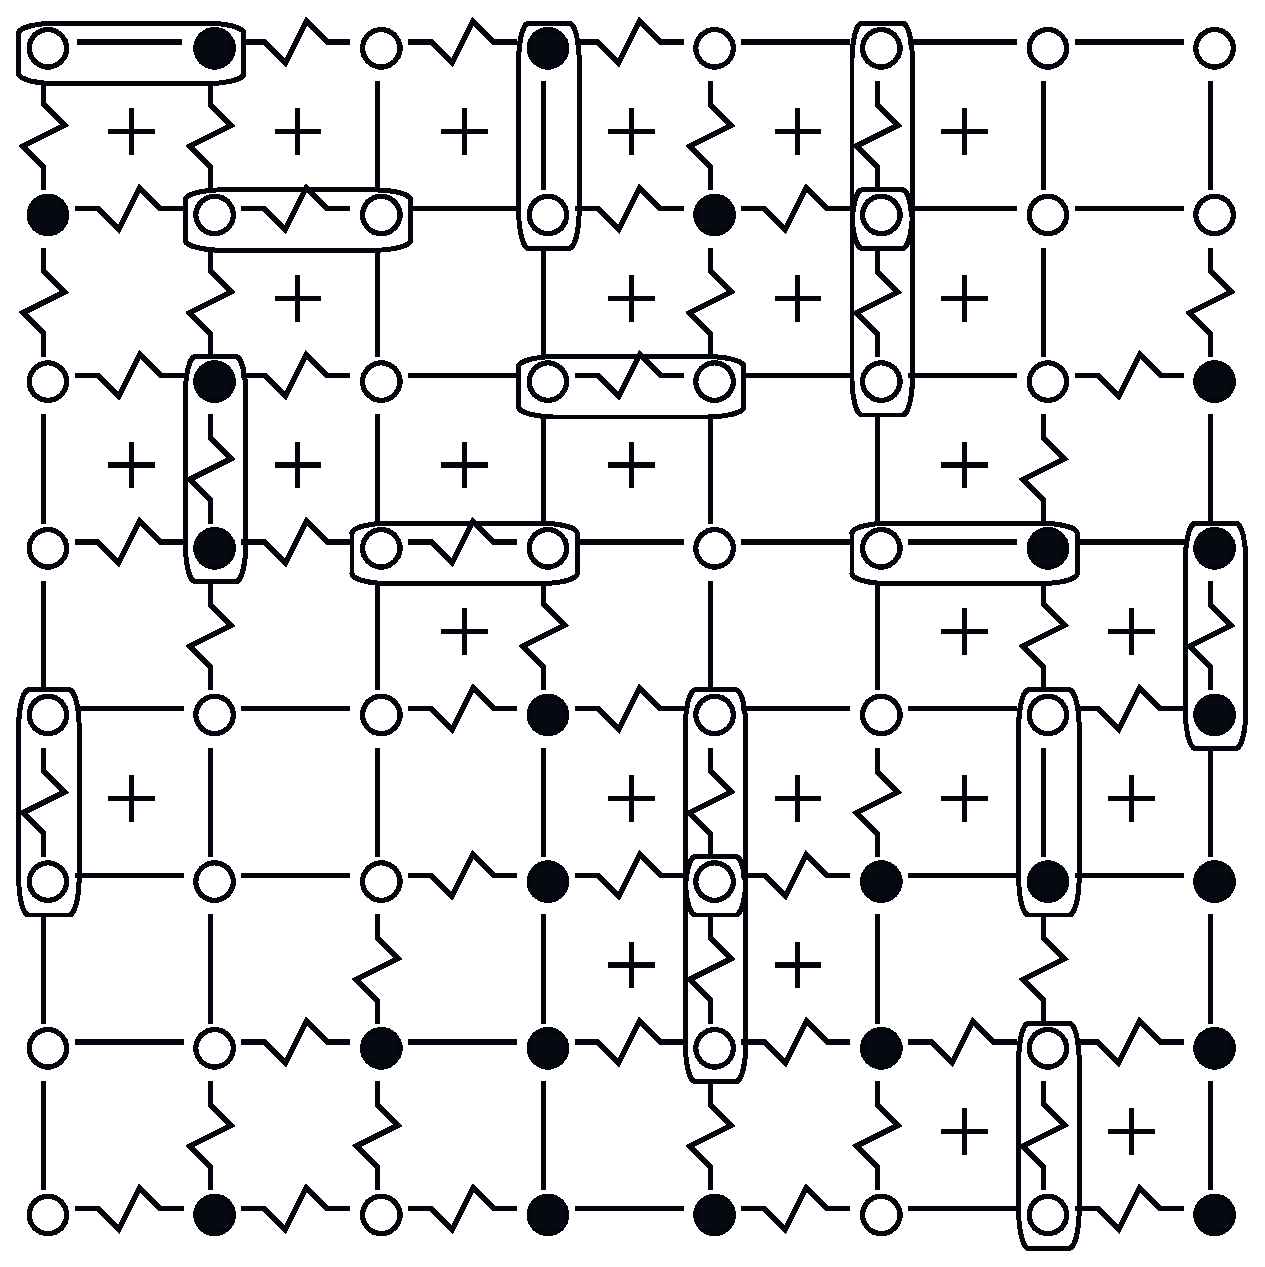
\includegraphics[width=1\linewidth]{pictures/SG_64_J0}
		\end{minipage}
		\hfill
		\begin{minipage}[h]{0.3\linewidth}
			\centering(c)
			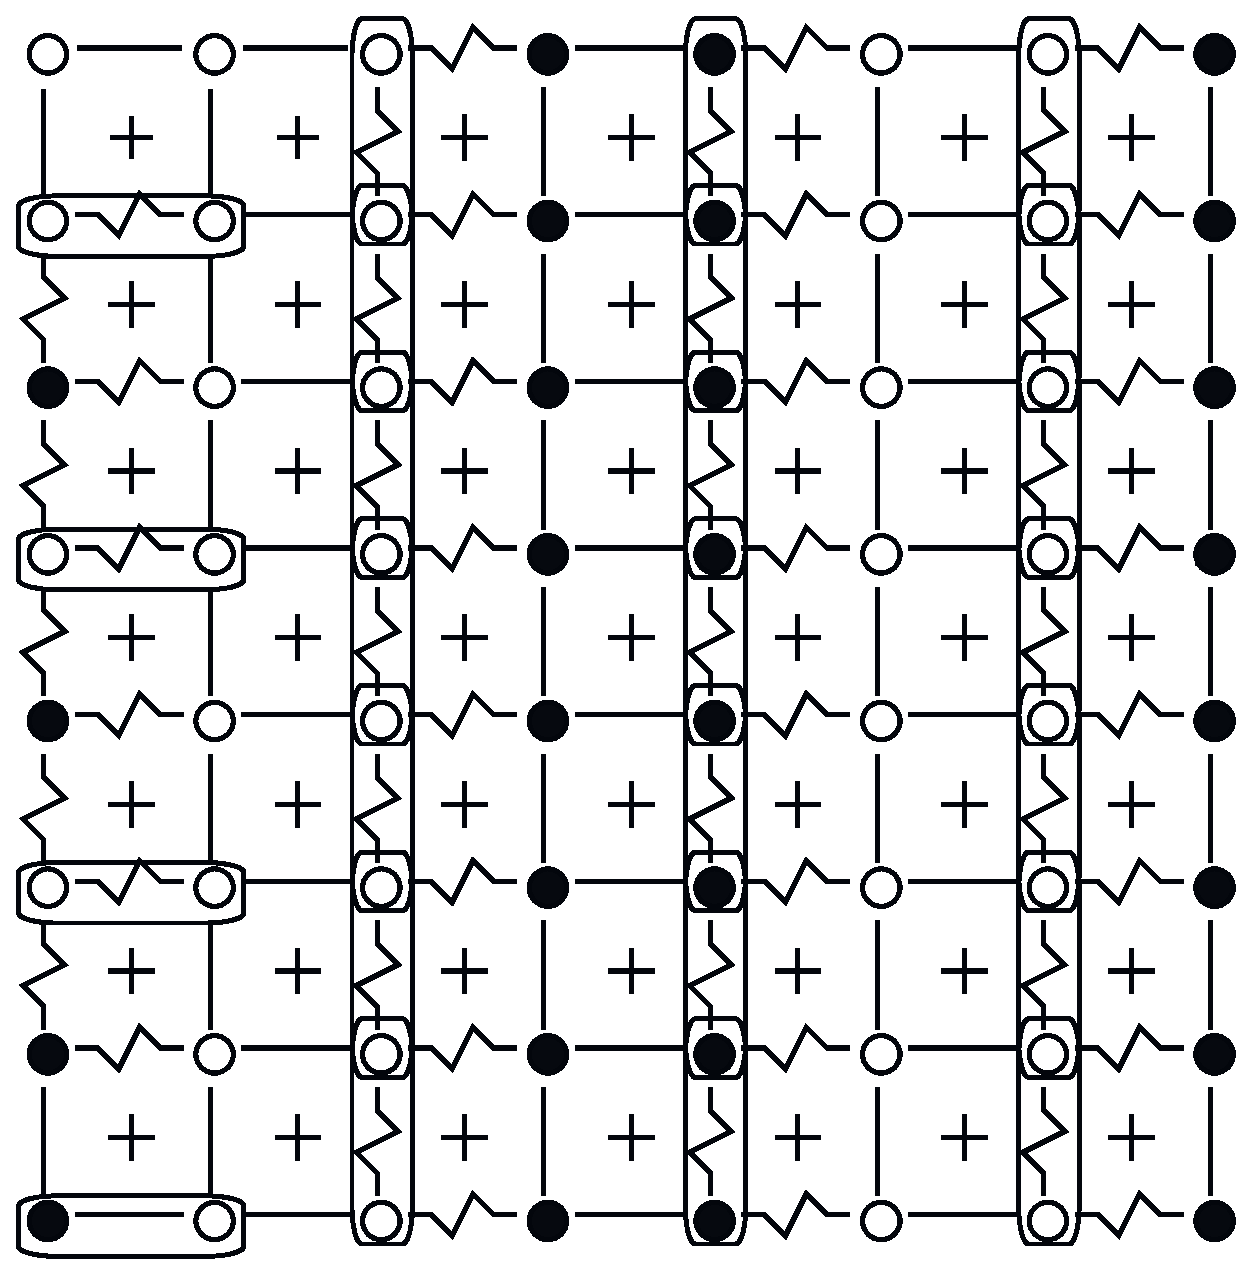
\includegraphics[width=1\linewidth]{pictures/SI_64_J0}
		\end{minipage}
		\hfill
		\caption{Exchange interactions, types of plaquettes, and ground state configurations of two-sublattice antiferromagnet (a), spin glass (b), and highly frustrated spin system (c) lattices consisting of 64 spins, $P_+ = 0.5$.}
		\label{fig:cell_SI_SG_64}
		
	\end{figure}
	

	The $\pm J$ periodicity condition does not always lead to macroscopic ground state degeneracy. In a two-sublattice antiferromagnet, there are no Type-II plaquettes (Figure~\ref{fig:cell_SI_SG_64}(a)).
	Spin glass differs from othes spin systems in that the exchange interactions are random, as illustrated in Figure~\ref{fig:cell_SI_SG_64}(b).
	Figure~\ref{fig:cell_SI_SG_64}(c) presents one of the many ground state spin configurations of a highly frustrated spin system. Despite the presence of frustrated plaquettes, this configuration cannot be classified as spin ice.

	In \cite{grigera2018entropy}, the authors study spin ice on a simple square lattice with additional interactions. Crossed ferromagnetic interactions within Type-I plaquettes (see Figure~\ref{fig:Type1}) are necessary to form four triangular plaquettes, allowing frustrated bonds. Each frustrated triangle will contain two ferromagnetic bonds and one antiferromagnetic bond. Without these additional crossing interactions, the system would resemble the configuration in Figure~\ref{fig:cell_SI_SG_64}(a).

	In Ref.~\cite{kato2022flux}, for the case of a fraction of ferromagnetic plaquettes $p_F = 0$, i.e., in the checkerboard spin ice all interactions within the plaquettes are antiferromagnetic. The additional diagonal antiferromagnetic interactions give rise to four triangular plaquettes that allow for frustration. Each frustrated triangle consists of three antiferromagnetic bonds. In the absence of these additional diagonal interactions, the system would correspond to a lattice of square antiferromagnetic Type-III plaquettes (see Fig.~\ref{fig:Type3}), in which frustration cannot occur.
	
	In the pyrochlore lattice~\cite{peretyatko2017interplay, otsuka2018husimi}, each tetrahedron consists of four antiferromagnetic triangles that allow for frustration. A tetrahedron can serve as a building block for constructing a 3D lattice. We assume that the method of frustrated plaquettes can be applied to artificial spin ice lattices with dipolar interactions~\cite{andriushchenko2019large, shevchenko2017effect}, including exotic lattice geometries~\cite{makarova2021low, shevchenko2022order, makarov2019numerical}. The absence of a method for minimizing a generalized Hamiltonian that allows for the existence of frustrated bonds between spins motivates the use of the frustrated plaquette method.
	
	Thus, Figures~\ref{fig:cell_SI_SG_64}(a)--\ref{fig:cell_SI_SG_64}(c) illustrate the cases of a two-sublattice antiferromagnet, a spin glass, and a highly frustrated spin system, respectively.
	There are many possible arrangements of $\pm J$, not only for $P_+=0.5$, but also for other values within the range $0.1<P_+<0.9$, that still yield a highly frustrated spin system.
	
	
	Calculations show that the ground state energy per spin at $P_+ = 0.5$ and in the absence of an external magnetic field for two-sublattice antiferromagnet and highly frustrated spin system is -1.75 and -0.97, Figures \ref{fig:cell_SI_SG_64}(a) and \ref{fig:cell_SI_SG_64}(c), respectively. The specific ground state energy of spin glass in the Edwards-Anderson model is -1.28.
	
	Figure \ref{fig:cell_SI_SG_64}(a) shows a planar lattice of two-sublattice antiferromagnet composed of Type-I plaquettes, completely free of frustrations.
	Figure \ref{fig:cell_SI_SG_64}(b) depicts a spin glass lattice containing 49 plaquettes, of which 16 are of the Type-I, 27 are of Type-II, and 6 are of the Type-III, with a total of 15 frustrations.
	In the highly frustrated spin system shown in Figure \ref{fig:cell_SI_SG_64}(c), the maximum quantity of frustrations in this example is achieved by filling the system with Type-II plaquettes, resulting in 25 frustrations across 49 plaquettes.
	
	The ground state depends not just on the lattice size and probability $P_+$ but also on the distribution of (anti)ferromagnetic interactions. This show at Figures \ref{fig:cell_SI_SG_64} and \ref{fig:_multiplot_SI_SG_64}. Figure \ref{fig:cell_SI_SG_64} shows three $P_+ = 0.5$ samples in the ground state, but with different distributions of ferromagnetic and antiferromagnetic bonds.
	
	The lattice energy in Figure \ref{fig:cell_SI_SG_64}(a) is equal to the sum of the energies of all interacting pairs, since frustrations are absent, equal to $-112|J|$.
	
	For the same $P_+ = 0.5$ with the random distribution of ferromagnetic-antiferromagnetic interactions of Figure \ref{fig:cell_SI_SG_64}(b), we observe 15 frustrations. So the energy will be equal to $E = -112 + 15\times2 = -82$, which coincides with the results of the complete enumeration.
	
	Figure \ref{fig:cell_SI_SG_64}(c) represents a special case where both interactions and the resulting frustrations are simultaneously ordered. Figure \ref{fig:cell_SI_SG_64}(c) represents a special case where both interactions and emergent frustrations are simultaneously ordered. The largest quantity of frustrations (25) leads to the highest ground state energy: $E = -112 + 2\times25 = -62$.
	

	\section{Ground state in an external magnetic field}

	\begin{figure}[H]
		\begin{minipage}[h]{0.32\linewidth}
			\centering
			\hspace{1cm}(a)
			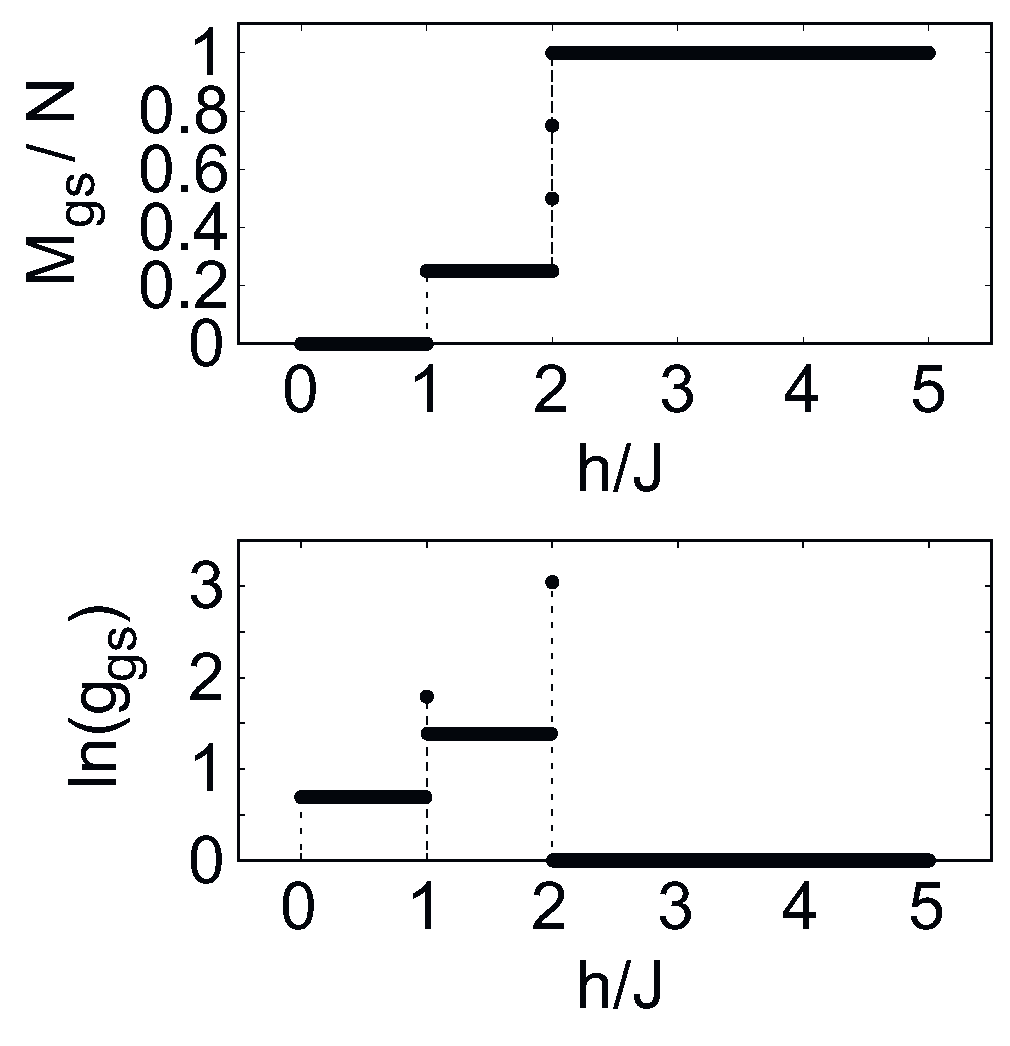
\includegraphics[width=1\linewidth]{pictures/_multiplot_SI64_J0_1}
		\end{minipage}
		\hfill
		\begin{minipage}[h]{0.32\linewidth}
			\centering
			\hspace{1cm}(b)
			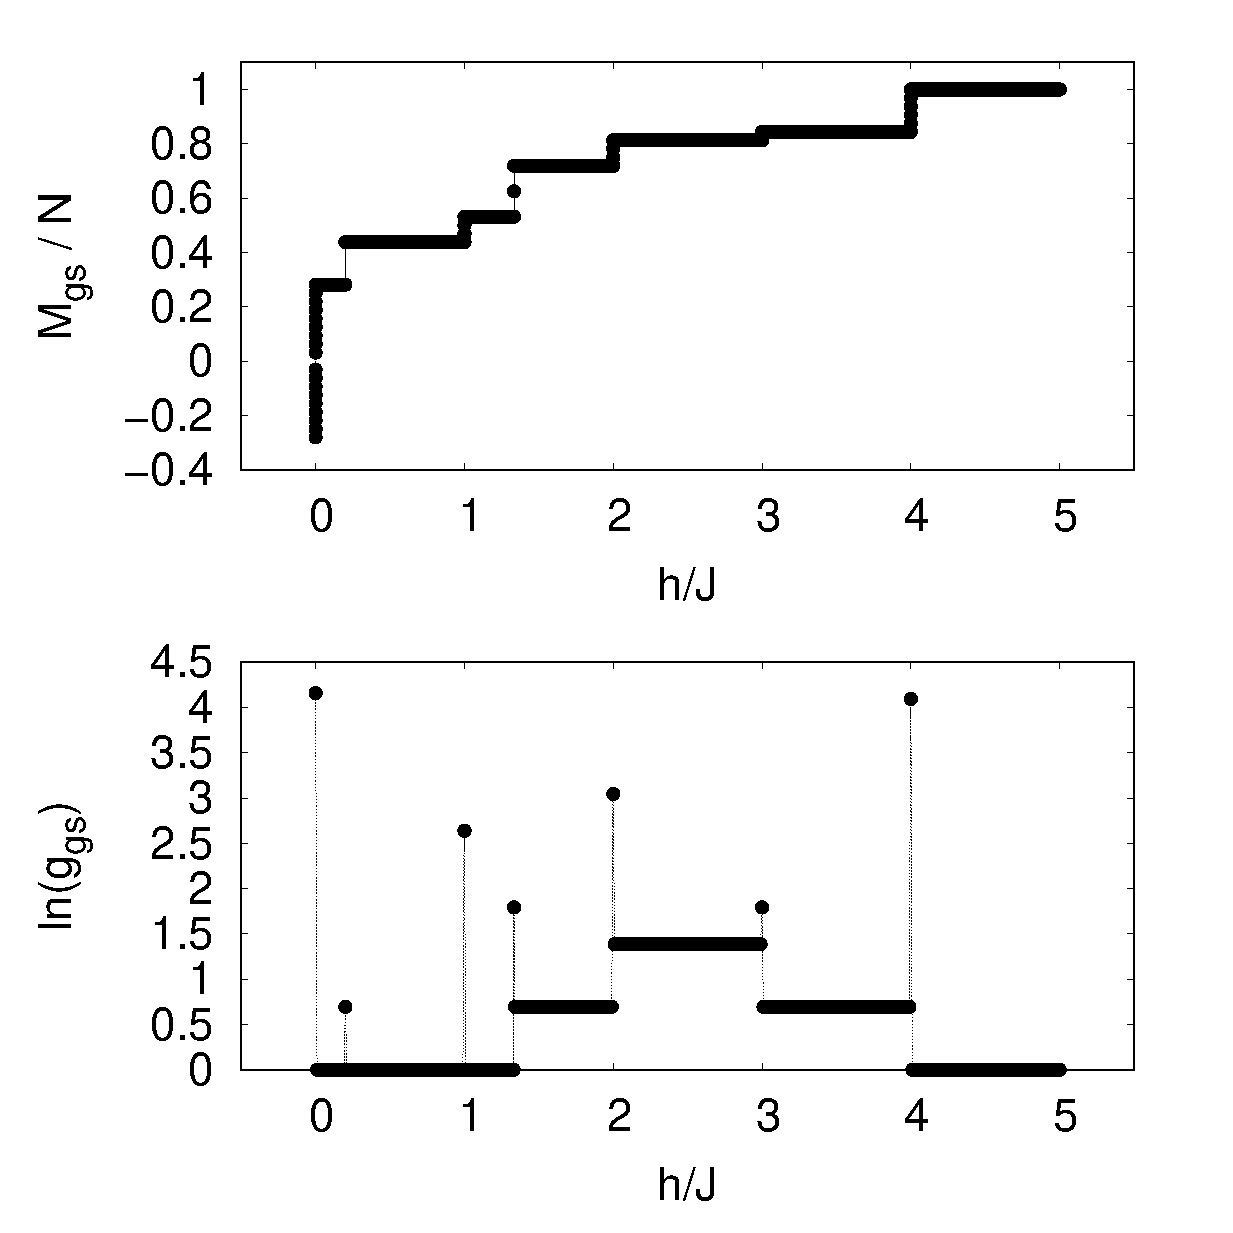
\includegraphics[width=1\linewidth]{pictures/_multiplot_SG64_J0}
		\end{minipage}
		\hfill
		\begin{minipage}[h]{0.32\linewidth}
			\centering
			\hspace{1cm}(c)
			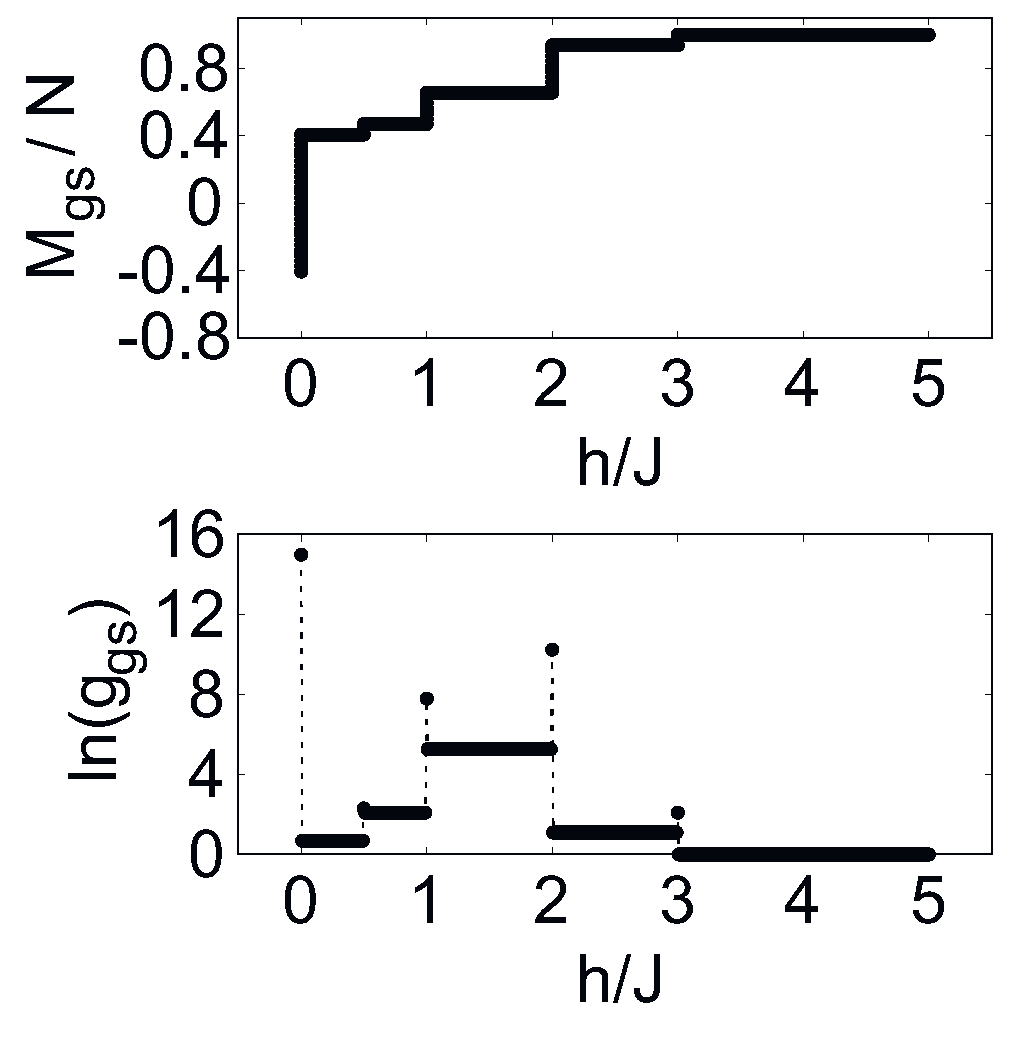
\includegraphics[width=1\linewidth]{pictures/_multiplot_SI64_J0}
		\end{minipage}
		
		\caption{Spin excess (upper panels) and residual entropy (lower panels) of two-sublattice antiferromagnet (a), spin glass (b) and highly frustrated spin system (c) (exchange constant distribution of $P_+ = 0.5$ shown in Figure \ref{fig:cell_SI_SG_64}).}
		\label{fig:_multiplot_SI_SG_64}
		
	\end{figure}

	Figure \ref{fig:_multiplot_SI_SG_64} shows the dependencies of spin excess and ground state degeneracy on the external magnetic field strength.
	In the absence of frustrations and an external magnetic field, the ground state of two-sublattice antiferromagnet is doubly degenerate (Figure \ref{fig:_multiplot_SI_SG_64}(a)).
	In spin glass, the frustrations increase the ground state degeneracy to 64 (Figure \ref{fig:_multiplot_SI_SG_64}(b)).
	Maximal filling of the highly frustrated spin system with frustrated Type-II plaquettes leads to macroscopic ground state degeneracy, with the number of degenerate configurations $> 3\times10^{6}$ (Figure \ref{fig:_multiplot_SI_SG_64}(c)).
	
	In Figure \ref{fig:_multiplot_SI_SG_64}(a), the spin excess is zero for the two configurations in the absence of frustrations and twofold degeneracy. The presence of frustrations in Figures \ref{fig:_multiplot_SI_SG_64}(b) and \ref{fig:_multiplot_SI_SG_64}(c) leads to the degeneracy of the ground state. The ground state configurations have spin excesses different from zero.
	
	As seen in Figures \ref{fig:_multiplot_SI_SG_64}(a)--\ref{fig:_multiplot_SI_SG_64}(c), the application of an external magnetic field leads to the emergence of steps (plateaus) in the behavior of the spin excess. The largest number of steps is observed for the spin glass (Figure \ref{fig:_multiplot_SI_SG_64}(b)). Despite the maximum quantity of frustrations in the highly frustrated spin system (Figure \ref{fig:_multiplot_SI_SG_64}(c)), the number of plateaus is lower than in Figure \ref{fig:_multiplot_SI_SG_64}(b). This is related to the shape of the density of states (DOS) distribution; see Figures \ref{fig:HDOS_ice_1}--\ref{fig:HDOS_ice}.
	
	Using complete enumeration method, the densities of states were calculated for the highly frustrated spin system and spin glass cases shown in Figure \ref{fig:cell_SI_SG_64}, as functions of external magnetic field strength (Figures \ref{fig:HDOS_ice_1}, \ref{fig:HDOS_glass}, and \ref{fig:HDOS_ice}).
	The system's energy under the influence of an external magnetic field was calculated using Equation \eqref{eq:ising_energy}.
	
	\begin{figure}[H]
		\centering
		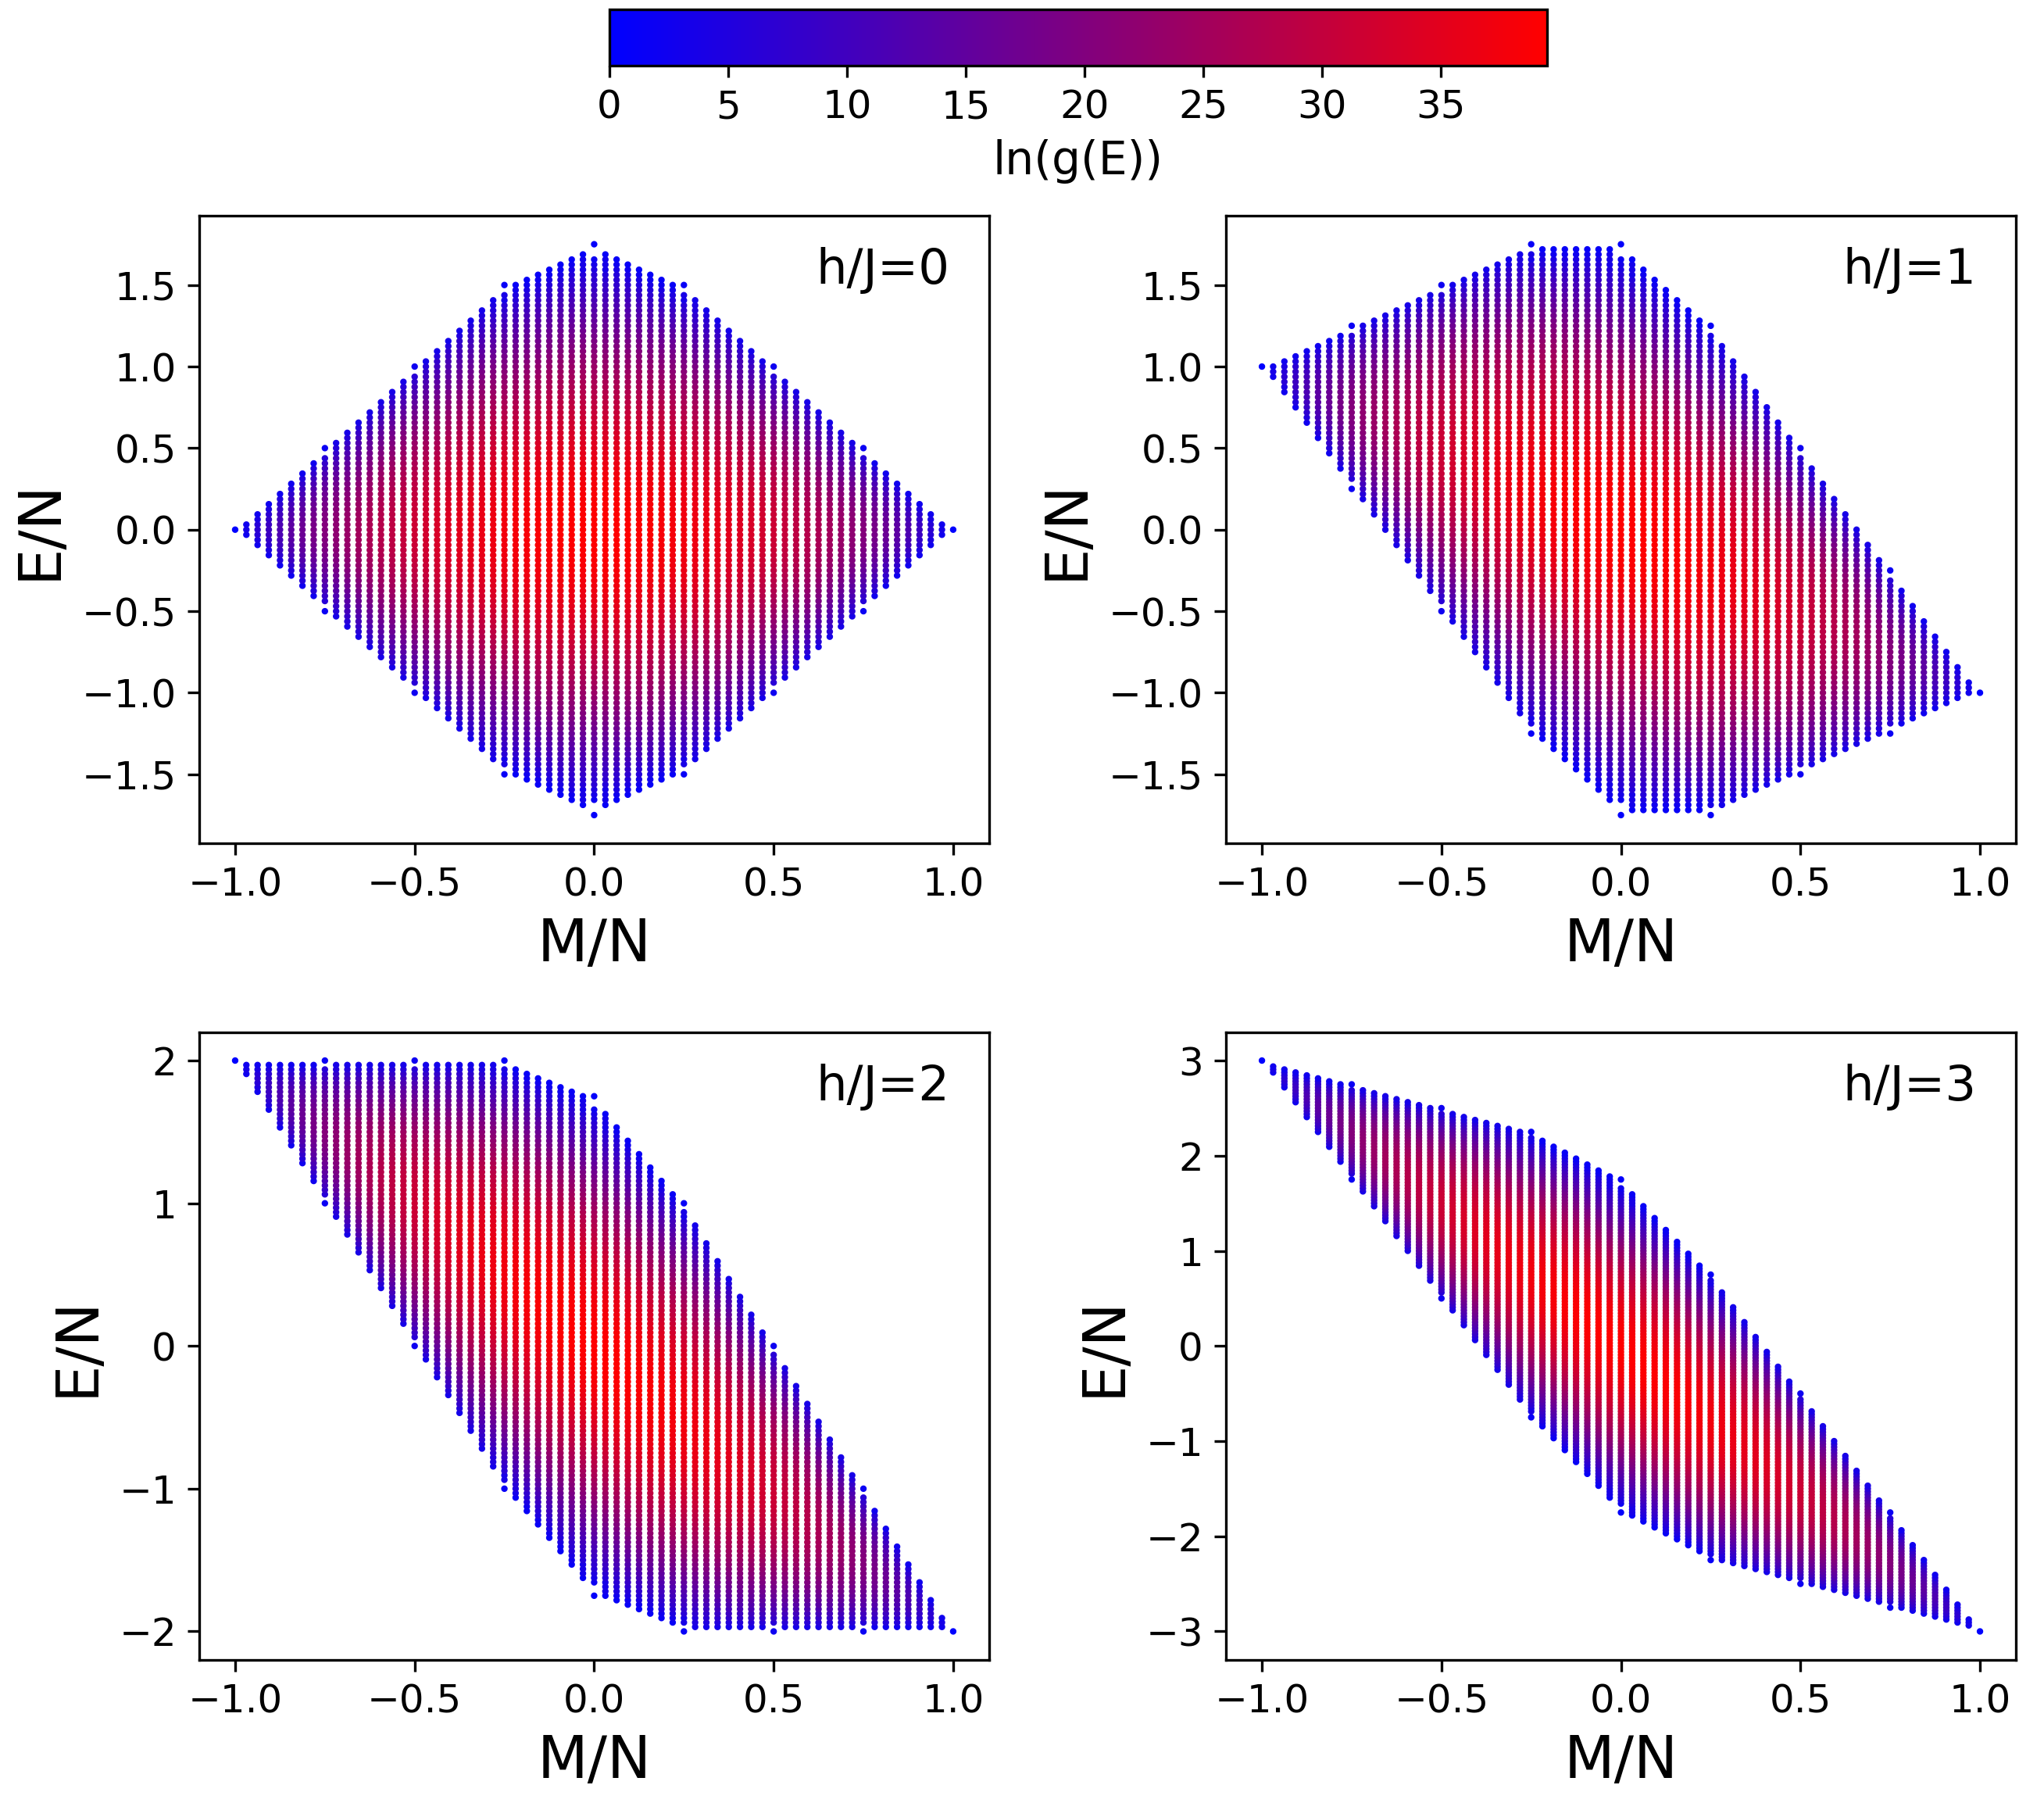
\includegraphics[width=1\linewidth]{pictures/HDOS_SI_64_J0_1.png}
		\caption{Density of states in an external magnetic field $0\leq h/J \leq 3$ for the two-sublattice antiferromagnet lattice (exchange constant distribution shown in Figure \ref{fig:cell_SI_SG_64}(a)), $P_+ = 0.5$. The plateau at $h/J=1$ arises due to free boundary conditions. The absence of Type-II plaquettes in a two-sublattice antiferromagnet leads to a spin reversal at an external field value of $h/J=2$. At this value of the critical field, the entropies of the states are summed.}
		\label{fig:HDOS_ice_1}
	\end{figure}
	
	\begin{figure}[H]
		\centering
		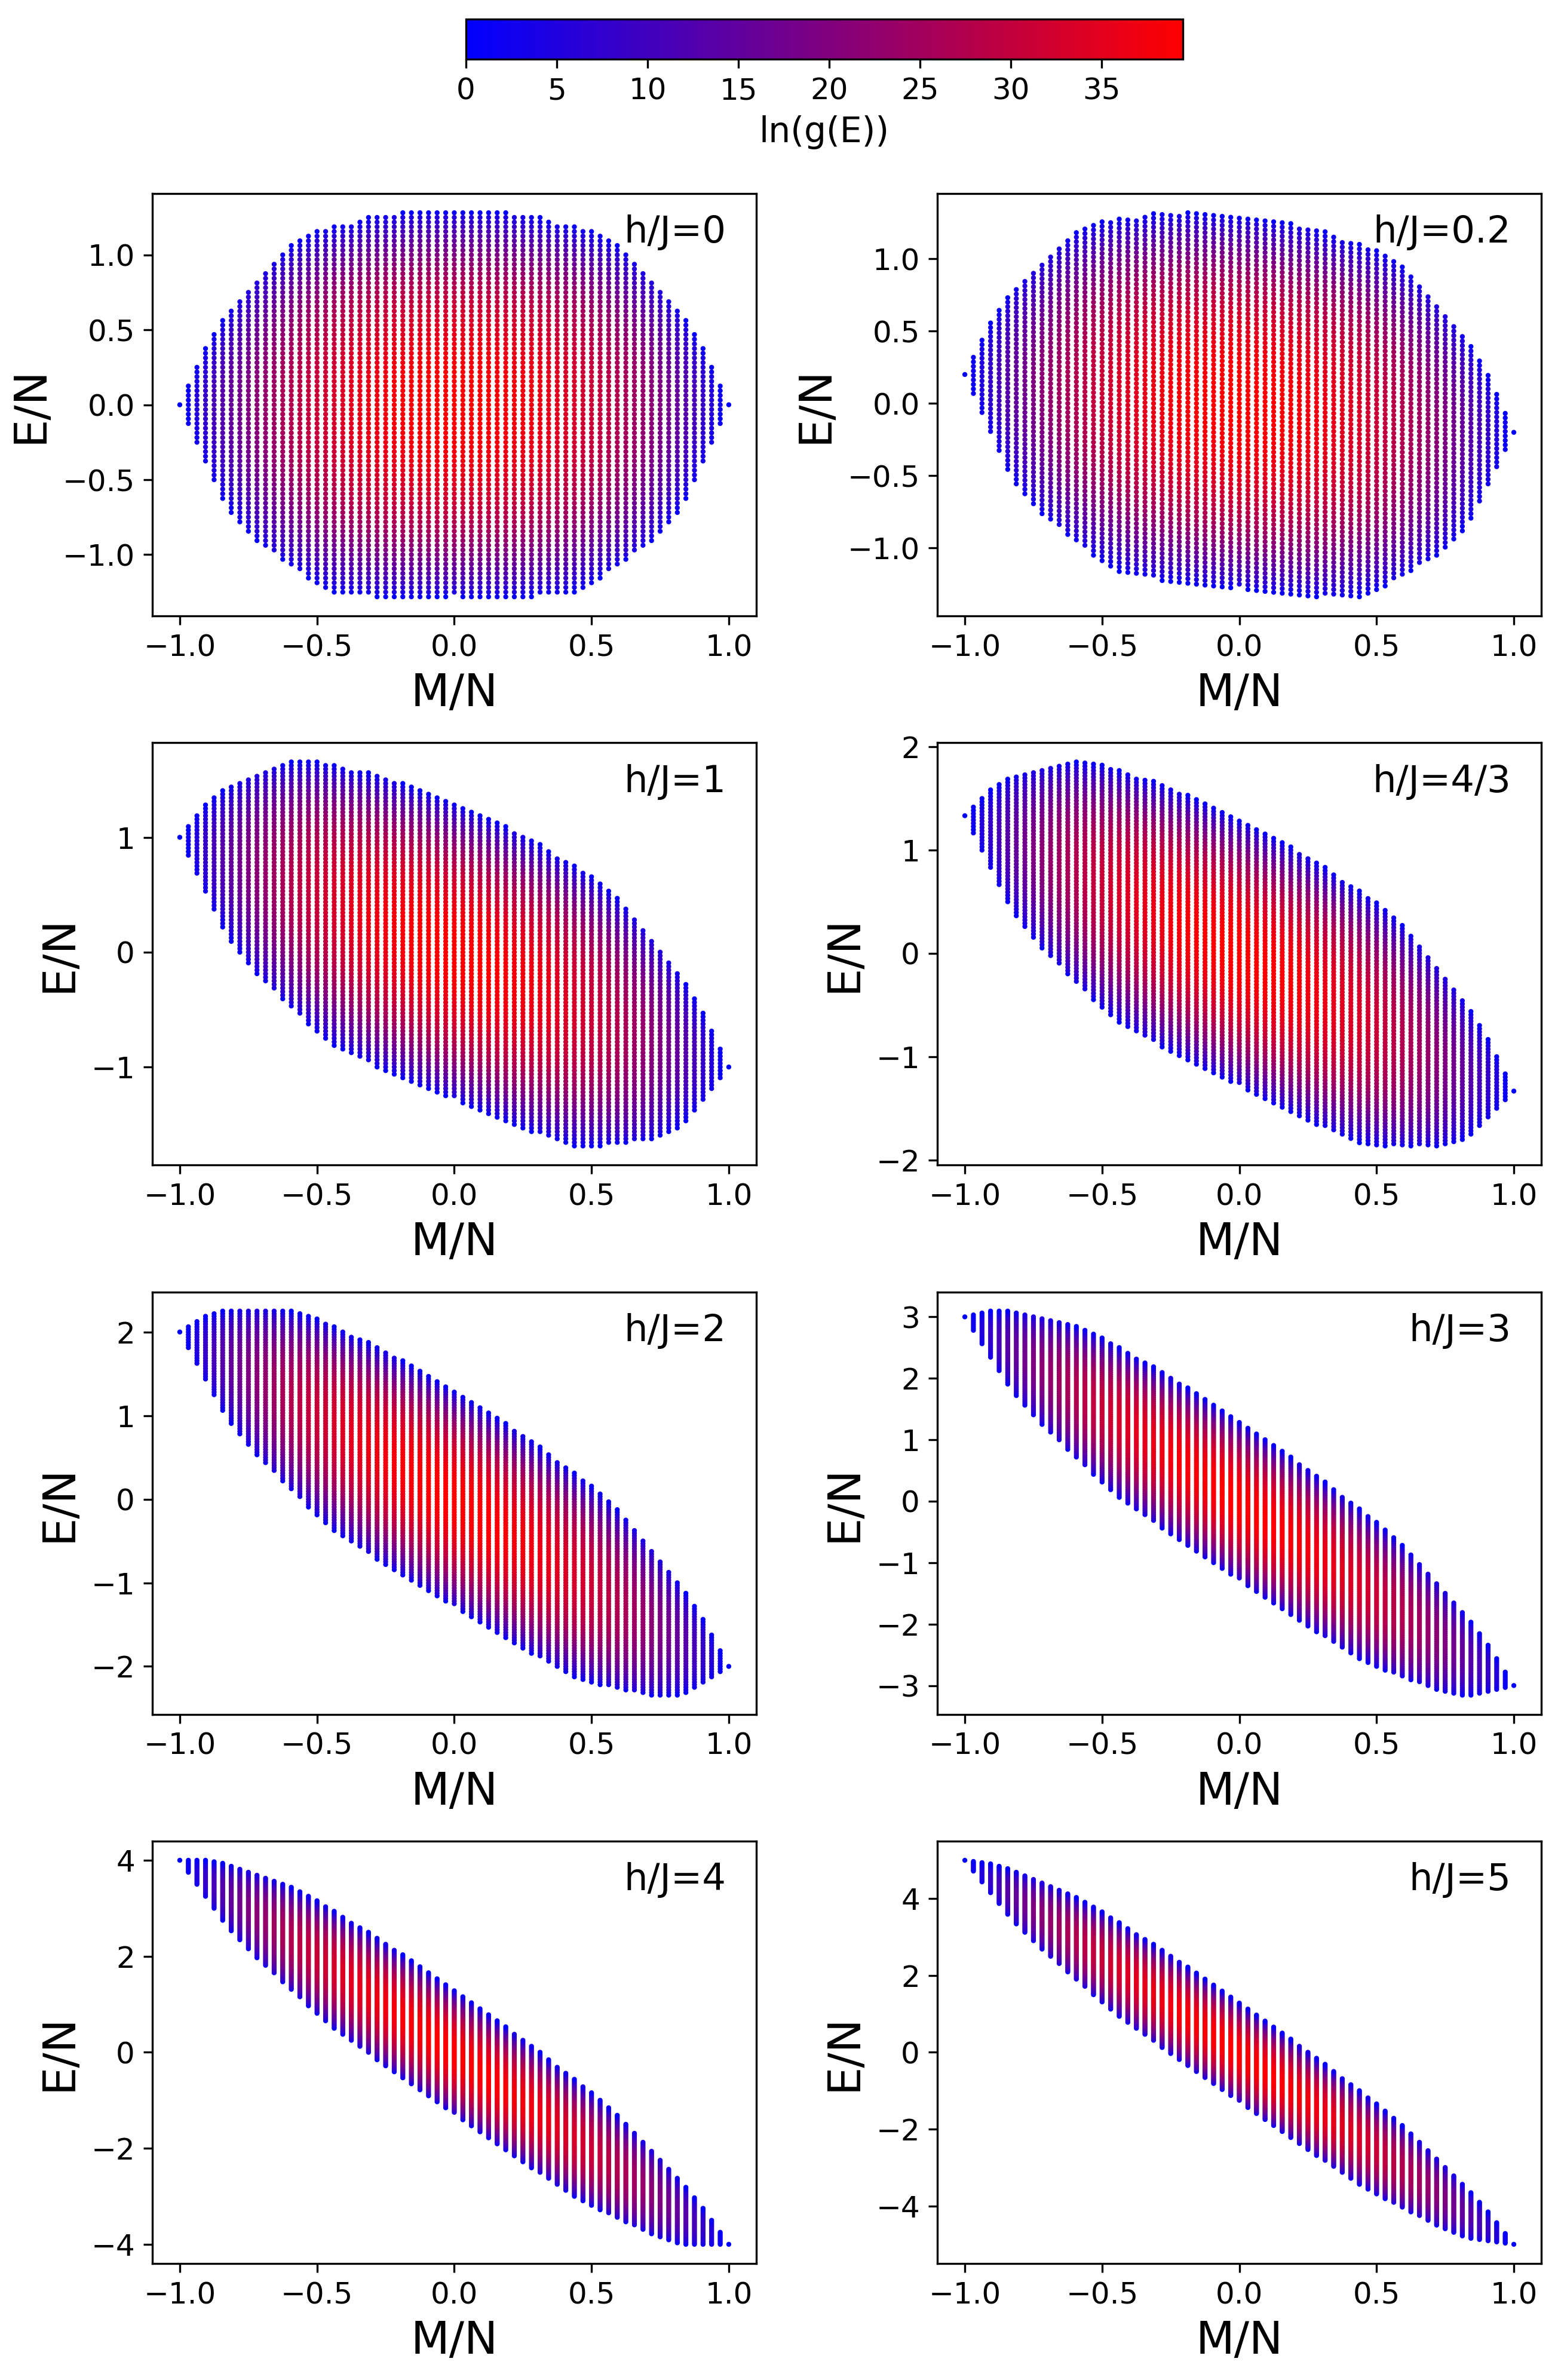
\includegraphics[width=1\linewidth]{pictures/HDOS_SG_64_J0.png}
		\caption{Density of states in an external magnetic field $0\leq h/J \leq 5$ for the spin glass lattice (exchange constant distribution shown in Figure \ref{fig:cell_SI_SG_64}(b)), $P_+ = 0.5$. There are 7 values of critical fields at which entropy peaks are observed.}
		\label{fig:HDOS_glass}
	\end{figure}
	
	
	\begin{figure}[H]
		\centering
		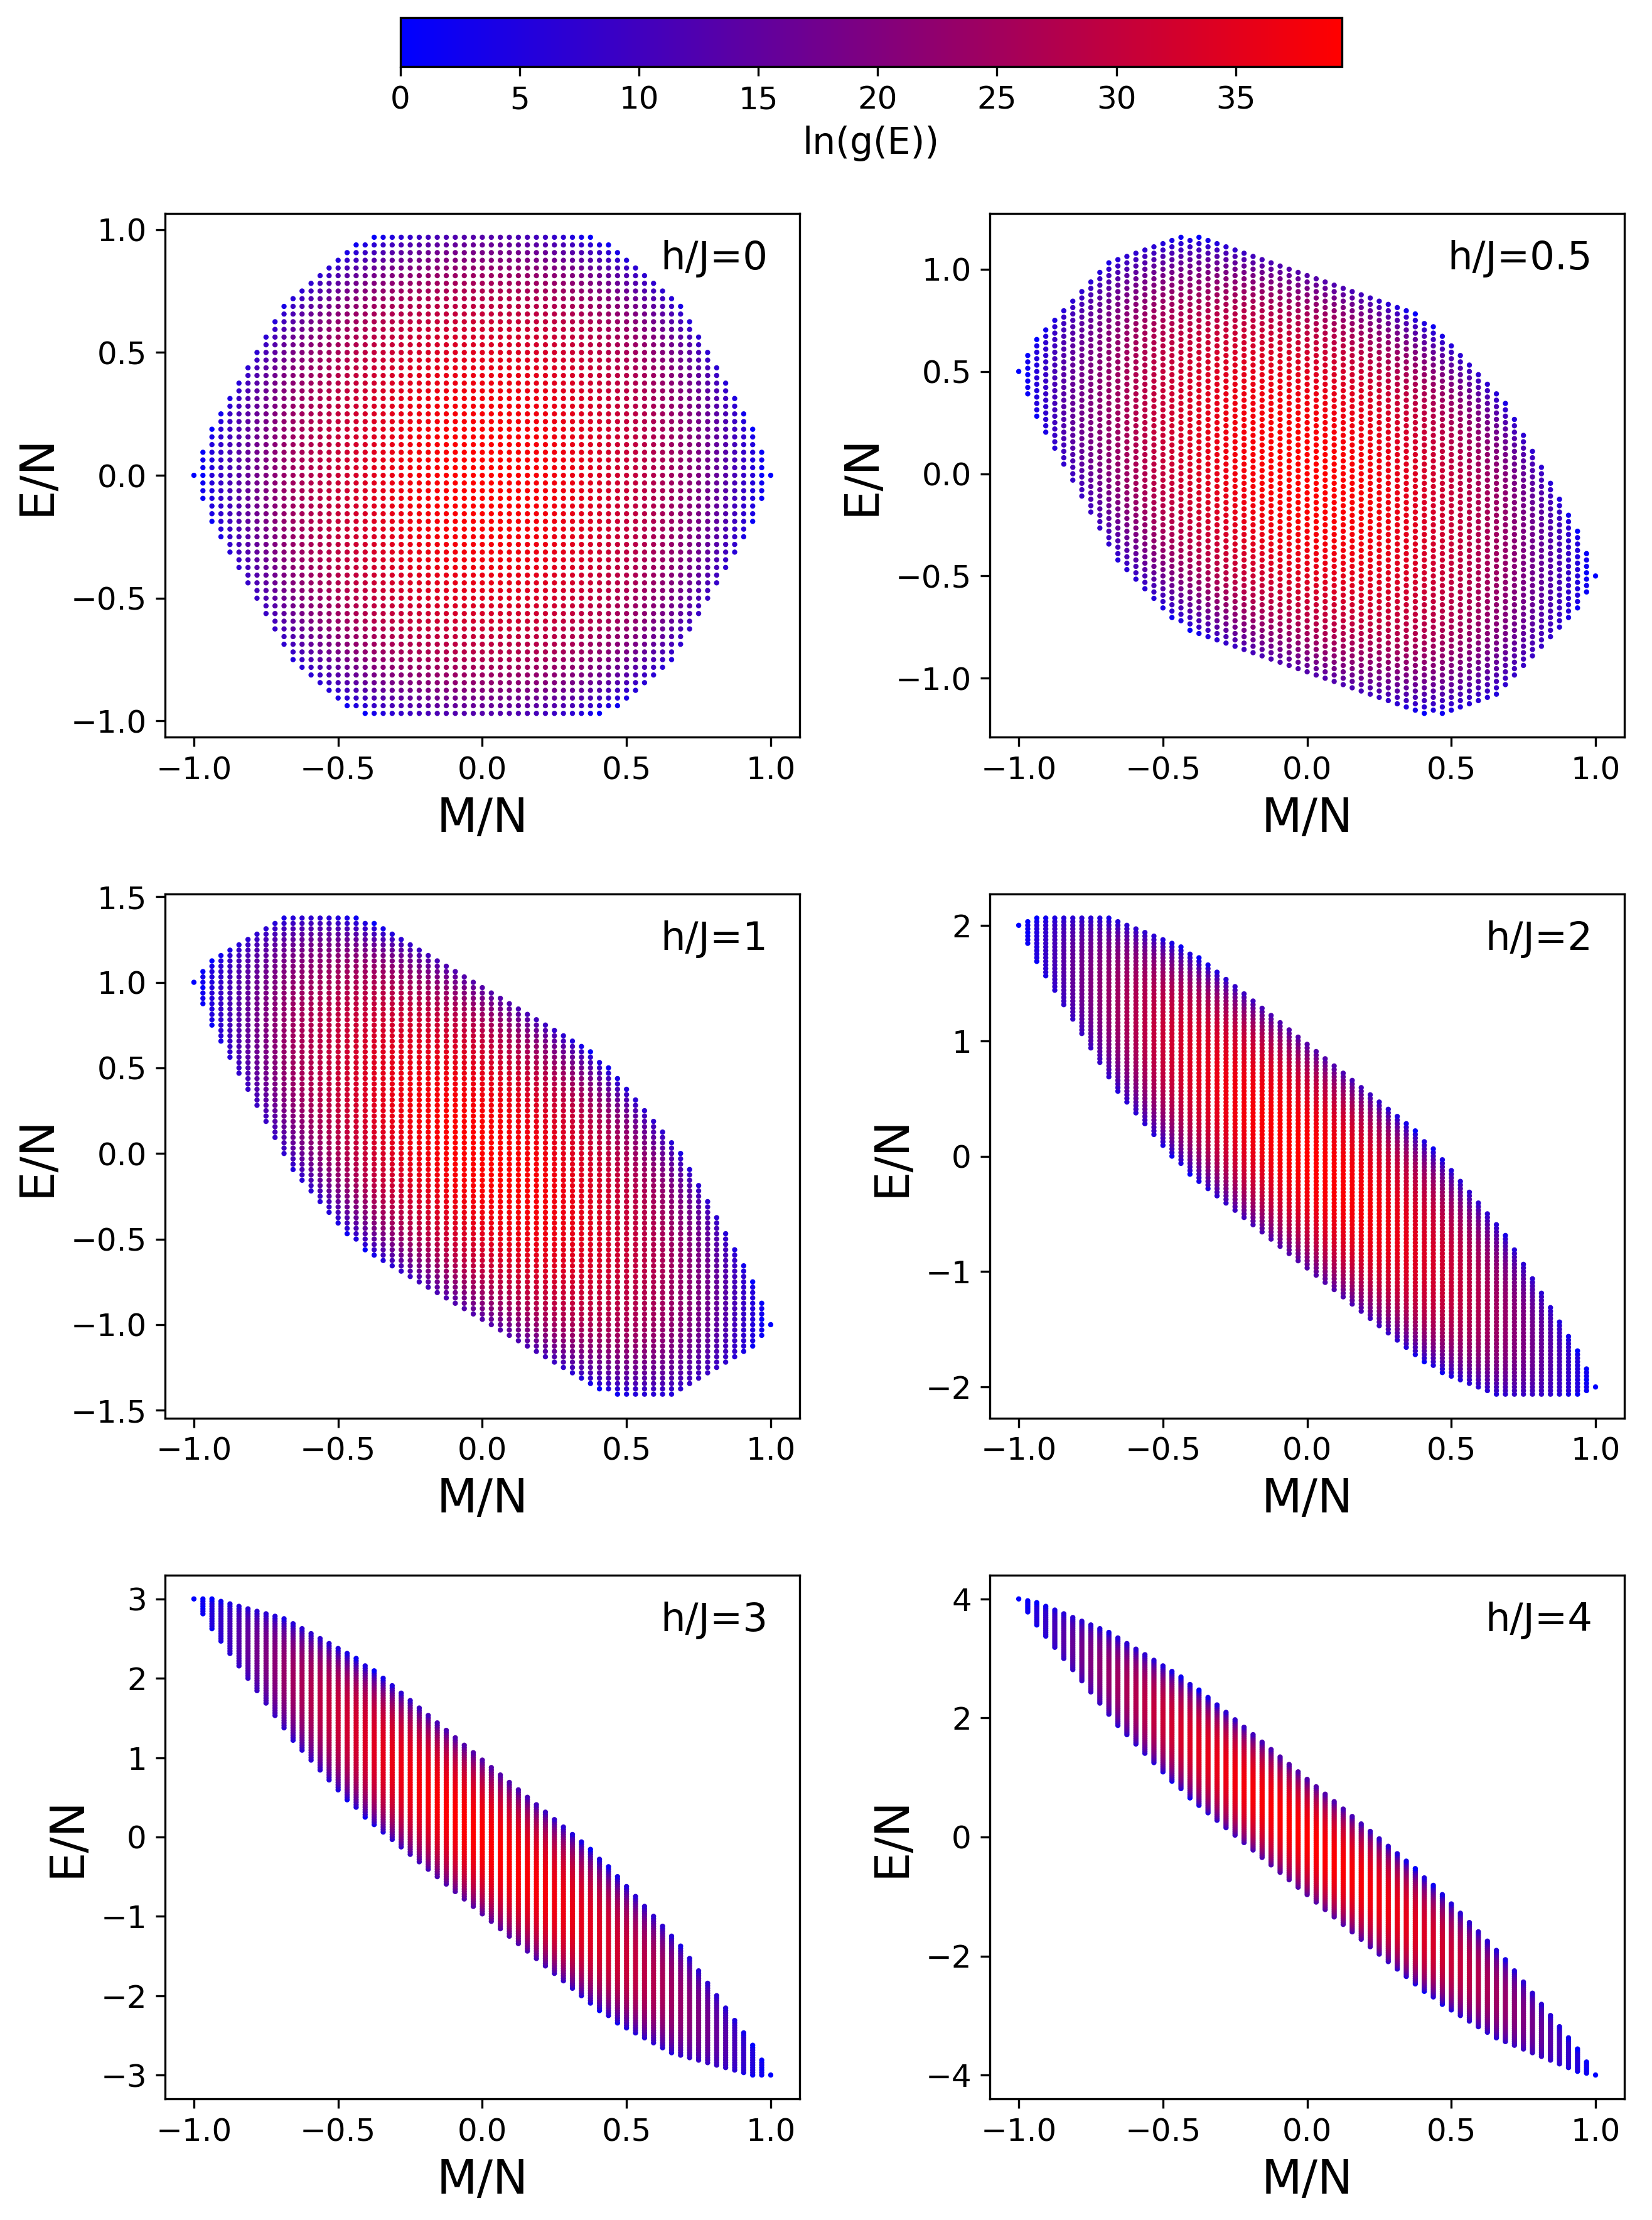
\includegraphics[width=1\linewidth]{pictures/HDOS_SI_64_J0.png}
		\caption{Density of states in an external magnetic field $0\leq h/J \leq 4$ for the highly frustrated spin system (exchange constant distribution shown in Figure \ref{fig:cell_SI_SG_64}(c)), $P_+ = 0.5$. The value $M=1$ is achieved at the critical field $h/J=3$. This value is lower for highly frustrated spin system than for spin glass.}
		\label{fig:HDOS_ice}
	\end{figure}
	
	In Figure \ref{fig:HDOS_ice_1}, at $h/J = 0$ for two-sublattice antiferromagnet (Figure \ref{fig:cell_SI_SG_64}(a)), a twofold degeneracy of the ground state can be observed. The external magnetic field value $h/J = 1$ is critical. At this field, the ground states with spin excess $M = 0$ and $M = 0.25$ have the same energy. This occurs due to the increasing contribution of the Zeeman energy, leading to the addition of the entropies of the ground states.  
	Increasing the external magnetic field to the critical value $h/J = 2$ results in a situation where the ground states correspond to spin excess values $M = 0.25, 0.5, 0.75, 1$. The degeneracies of these four states add up, leading to a higher entropy peak than at $h/J = 1$.  
	The value $h/J = 3$ corresponds to the saturation field, at which only a single configuration remains.
	
	For the spin glass (Figure \ref{fig:cell_SI_SG_64}(b)), entropy peaks at $T = 0$ in critical fields are determined by the boundaries of the density of states (see Figure \ref{fig:HDOS_glass}).
	Highly frustrated spin system (Figure \ref{fig:cell_SI_SG_64}(c)) exhibits a lower diversity of critical fields compared to the spin glass (see Figure \ref{fig:HDOS_ice}). However, the degeneracy of the ground states is higher than in the spin glass.
	The presence of Type-I, Type-II, and Type-III plaquettes in the spin glass (Figure \ref{fig:cell_SI_SG_64}(b)) leads to a wide variety of critical field values. In the two-sublattice antiferromagnet (Figure \ref{fig:cell_SI_SG_64}(a)), there were only Type-I plaquettes, while in highly frustrated spin system (Figure \ref{fig:cell_SI_SG_64}(c)), only Type-II plaquettes were present.
	
	An important conclusion is that Figures \ref{fig:HDOS_ice_1}--\ref{fig:HDOS_ice} clearly illustrate the emergence of entropy peaks in Figure \ref{fig:_multiplot_SI_SG_64} and the formation of plateaus in the dependence of spin excess on the external magnetic field.  
	The quantity of critical fields (including $h/J=0$) in Figures \ref{fig:HDOS_ice_1}, \ref{fig:HDOS_glass}, and \ref{fig:HDOS_ice} matches the number of plateaus in Figures \ref{fig:_multiplot_SI_SG_64}(a), \ref{fig:_multiplot_SI_SG_64}(b), and \ref{fig:_multiplot_SI_SG_64}(c), respectively.
	
	
	\section{Antiferromagnetism, spin glass, and ferromagnetism at $T = 0$}
	
	The phase diagram at non-zero temperatures in an external magnetic field was studied in \cite{trukhin2024thermodynamic}. Of particular interest is the separation of antiferromagnetic, spin glass, and ferromagnetic states at $T = 0$.
	
	Table \ref{tab:lit_phase} summarizes theoretical and numerical results for the critical transition point (relative concentration of ferromagnetic bonds $P_+$) from the antiferromagnetic state to the spin glass state.
	
	\begin{table}[!h]
		\centering
		\begin{tabular}{|l|c|l|}
			\hline
			Method & \( P_{+} \) & Reference \\ \hline
			Series expansion & ~0.099 & \cite{PhysRevB.19.260} \\ \hline
			Matching algorithm & \( 0.105 \pm 0.01 \) & \cite{H_Freund_1989} \\ \hline
			Matching algorithm & \( 0.095 < p_c < 0.108 \) & \cite{BENDISCH1994139} \\ \hline
			Exact ground states & \( 0.106 \pm 0.002 \) & \cite{N.Kawashima_1997} \\ \hline
			Ground state enumeration & 0.115 & \cite{PhysRevE.58.1502} \\ \hline
			Exact ground states & \( 0.1031 \pm 0.0001 \) & \cite{WANG200331} \\ \hline
			Exact ground states & \( 0.103 \pm 0.001 \) & \cite{amoruso2004domain} \\ \hline
		\end{tabular}
		\caption{Critical point for the concentration AFM-SG transition (ferromagnetic bond concentration $ P_+ $).}
		\label{tab:lit_phase}
	\end{table}
	
	Figure \ref{fig:Mgs(P+)} shows the dependence of the maximum spin excess for the ground state on the relative number of ferromagnetic bonds $P_+$. The density of ferromagnetic bonds is determined by $P_+$, and bonds are randomly distributed. Each series consisted of 10 samples for numerical calculations for given $P_+$.
	
	\begin{figure}[H]
		\centering
		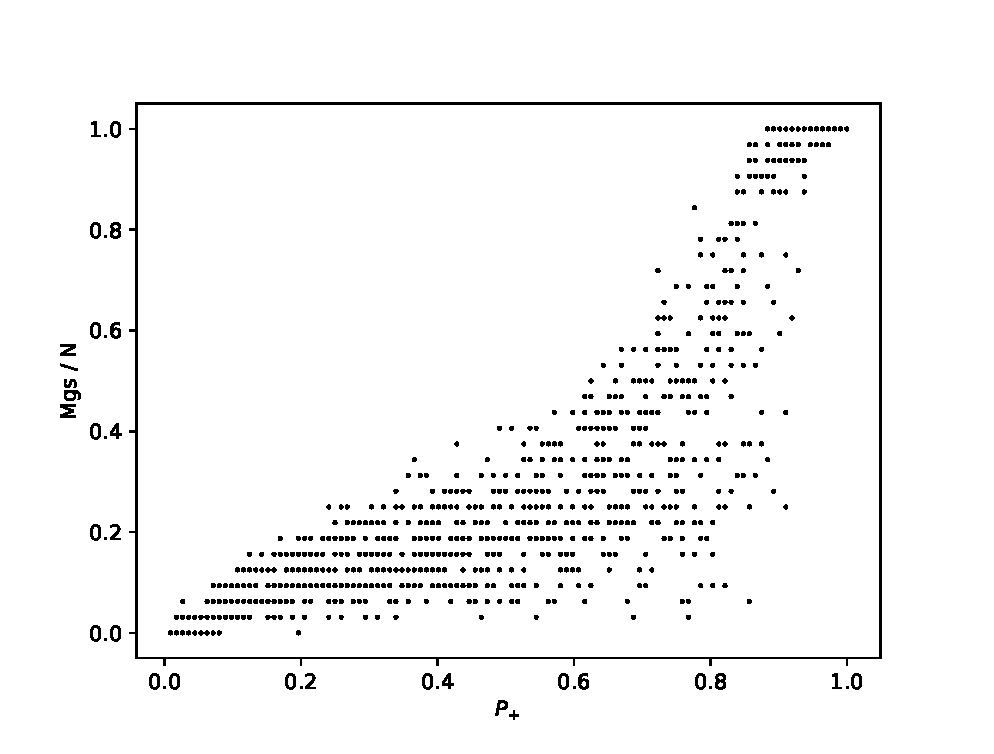
\includegraphics[width=0.8\textwidth]{images/Mgs(P+).eps}
		\caption{Maximum ground state spin excess as a function of the relative number of ferromagnetic bonds $P_+$.}
		\label{fig:Mgs(P+)}
	\end{figure}
	
	Let $M_{gs}$ -- the absolute value of a maximum spin excess of the ground state. For a pure ferromagnet $P_+ = 1.0$, the spin excess of ground state equals $M_{gs}/N = 1.0$. In a pure antiferromagnet $P_+ = 0.0$, the spin excess of ground state equals $M_{gs}/N = 0.0$ (in the case of an even number of spins). Thus, if
		
	\begin{equation}
		M_{gs}/N = 1.0,
		\label{eq:ferr_deffinition}
	\end{equation}
		
	\noindent the sample is considered as ferromagnet, if
	
	\begin{equation}
		M_{gs}/N = 0.0,
		\label{eq:aferr_deffinition}
	\end{equation}
	
	\noindent the sample as antiferromagnet.
	
	For each $P_+$ value, the set of 10 samples was considered. The probability of ferromagnetic state $P_{FM}$ is defined as relative number of ferromagnetic samples in set, Figure \ref{fig:P_AFM_FM_Mmax}(b). Similarly, relative number of antiferromagnetic samples in set is the probability $P_{AFM}$, Figure \ref{fig:P_AFM_FM_Mmax}(a).
	
	\begin{figure}[H]
		\begin{minipage}[h]{0.45\linewidth}
			\centering (a)
			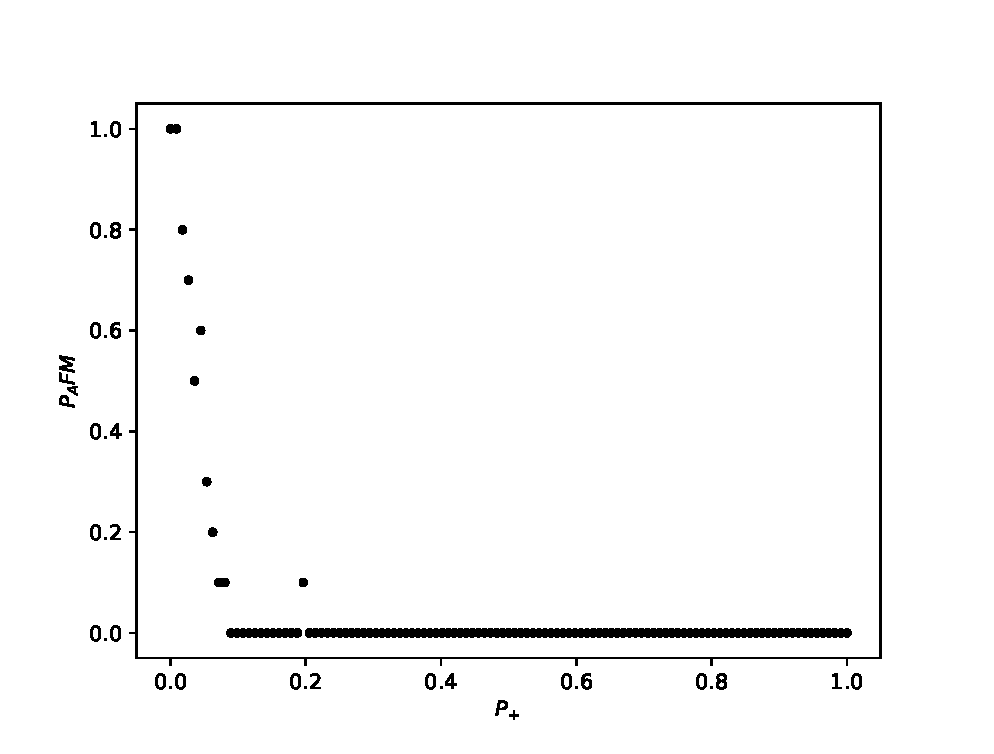
\includegraphics[width=1\linewidth]{images/P_AFM_Mmax.eps}
		\end{minipage}
		\hfill
		\begin{minipage}[h]{0.45\linewidth}
			\centering (b)
			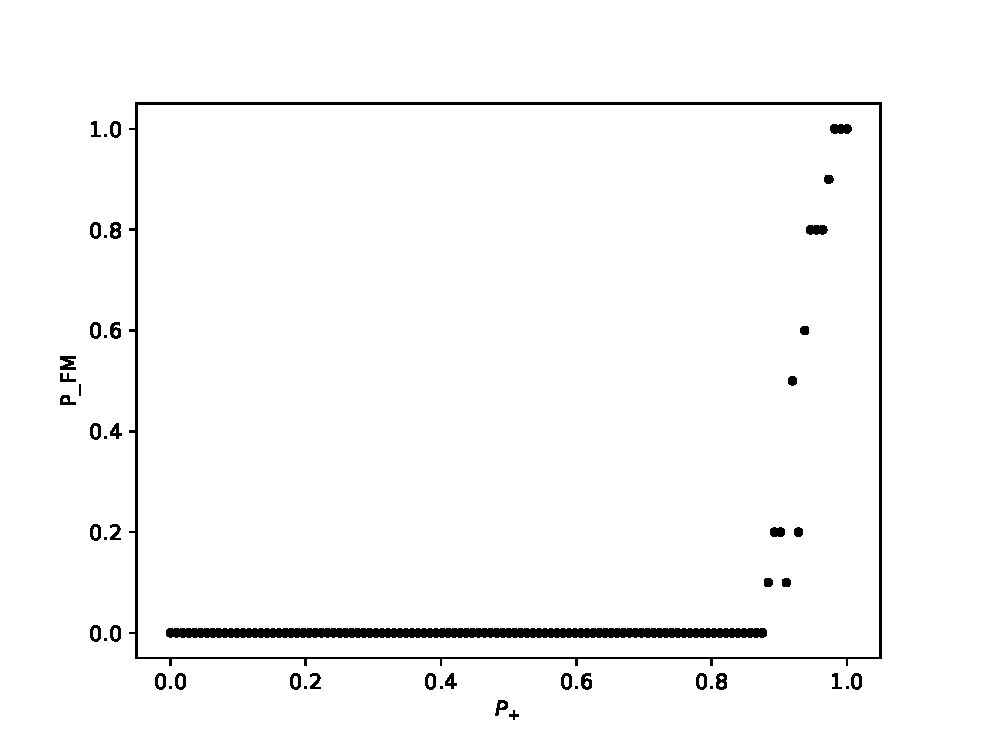
\includegraphics[width=1\linewidth]{images/P_FM_Mmax.eps}
		\end{minipage}
		\caption{Probability of antiferromagnetic (a) and ferromagnetic (b) states at \( T = 0 \).}
		\label{fig:P_AFM_FM_Mmax}
	\end{figure}
	
	The antiferromagnetic state at $T = 0$ occurs for $0.0 \leq P_+ \leq 0.1$. The spin glass state is realized for $0.1 \leq P_+ \leq 0.9$. The ferromagnetic state occurs for $0.9 \leq P_+ \leq 1.0$. The critical values for the antiferromagnetic state and for the ferromagnetic state at zero temperature in the absence of an external magnetic field are in Table \ref{tab:lit_phase}.
	
	The calculated full density of states allows to research of sample properties in an external magnetic field. Under an external magnetic field ($h/J = 1$ and $h/J = 2$, for example), the proportion of the ferromagnetic state increases while that of the antiferromagnetic state decreases, as shown in Figure \ref{fig:Mgs(P+)_H}. Phase transition points under an external field exhibit behavior similar to \cite{trukhin2024thermodynamic}.
	
	\begin{figure}[H]
		\begin{minipage}[h]{0.45\linewidth}
			\centering (a)
			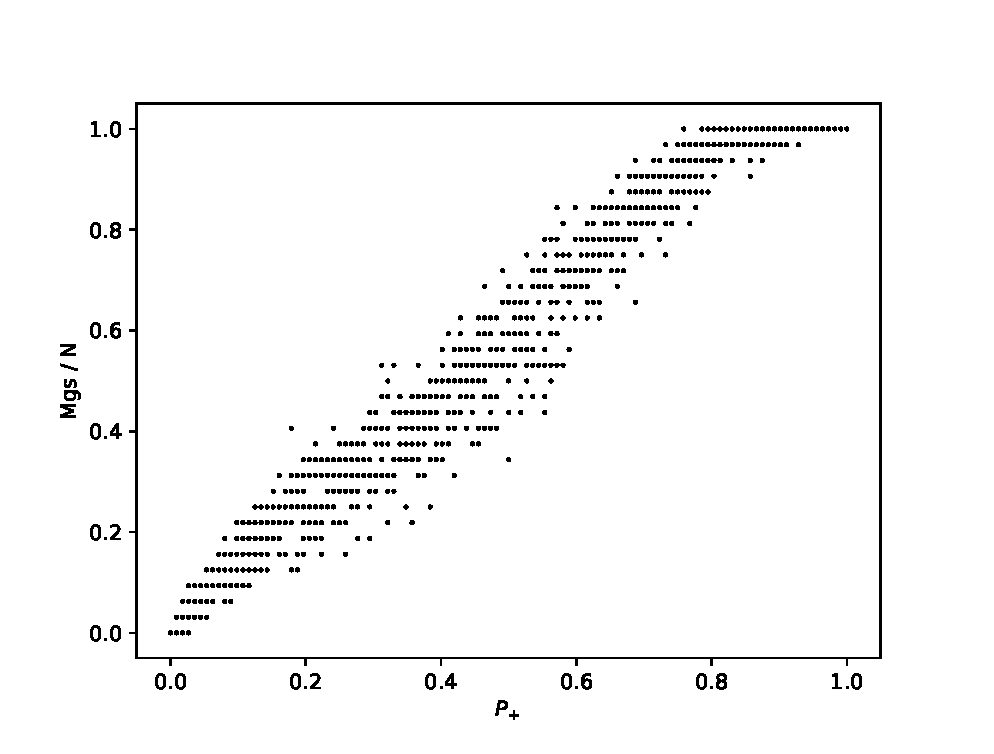
\includegraphics[width=1\linewidth]{images/Mgs(P+)_H1.eps}
		\end{minipage}
		\hfill
		\begin{minipage}[h]{0.45\linewidth}
			\centering (b)
			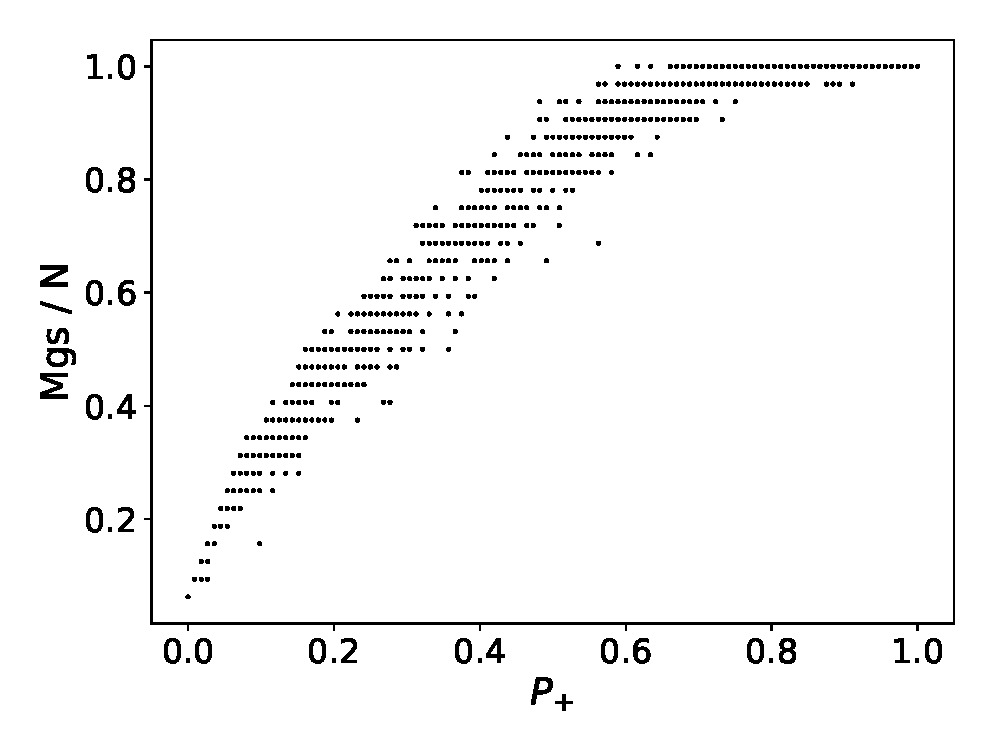
\includegraphics[width=1\linewidth]{images/Mgs(P+)_H2.eps}
		\end{minipage}
		\caption{Ground state spin excess for all values of bond distribution density under external fields $h/J = 1$ (a) and $h/J = 2$ (b).}
		\label{fig:Mgs(P+)_H}
	\end{figure}
	
	The theoretical ground state phase diagram ($h-P_+$) is shown in Figure \ref{fig:P+_afm_fm(H)}. Both Figure \ref{fig:Mgs(P+)_H} and Figure \ref{fig:P+_afm_fm(H)} were constructed based on the definitions of probability of ferromagnetism (Equation \eqref{eq:ferr_deffinition}) and antiferromagnetism (Equation \eqref{eq:aferr_deffinition}.)
	
	\begin{figure}[H]
		\centering
		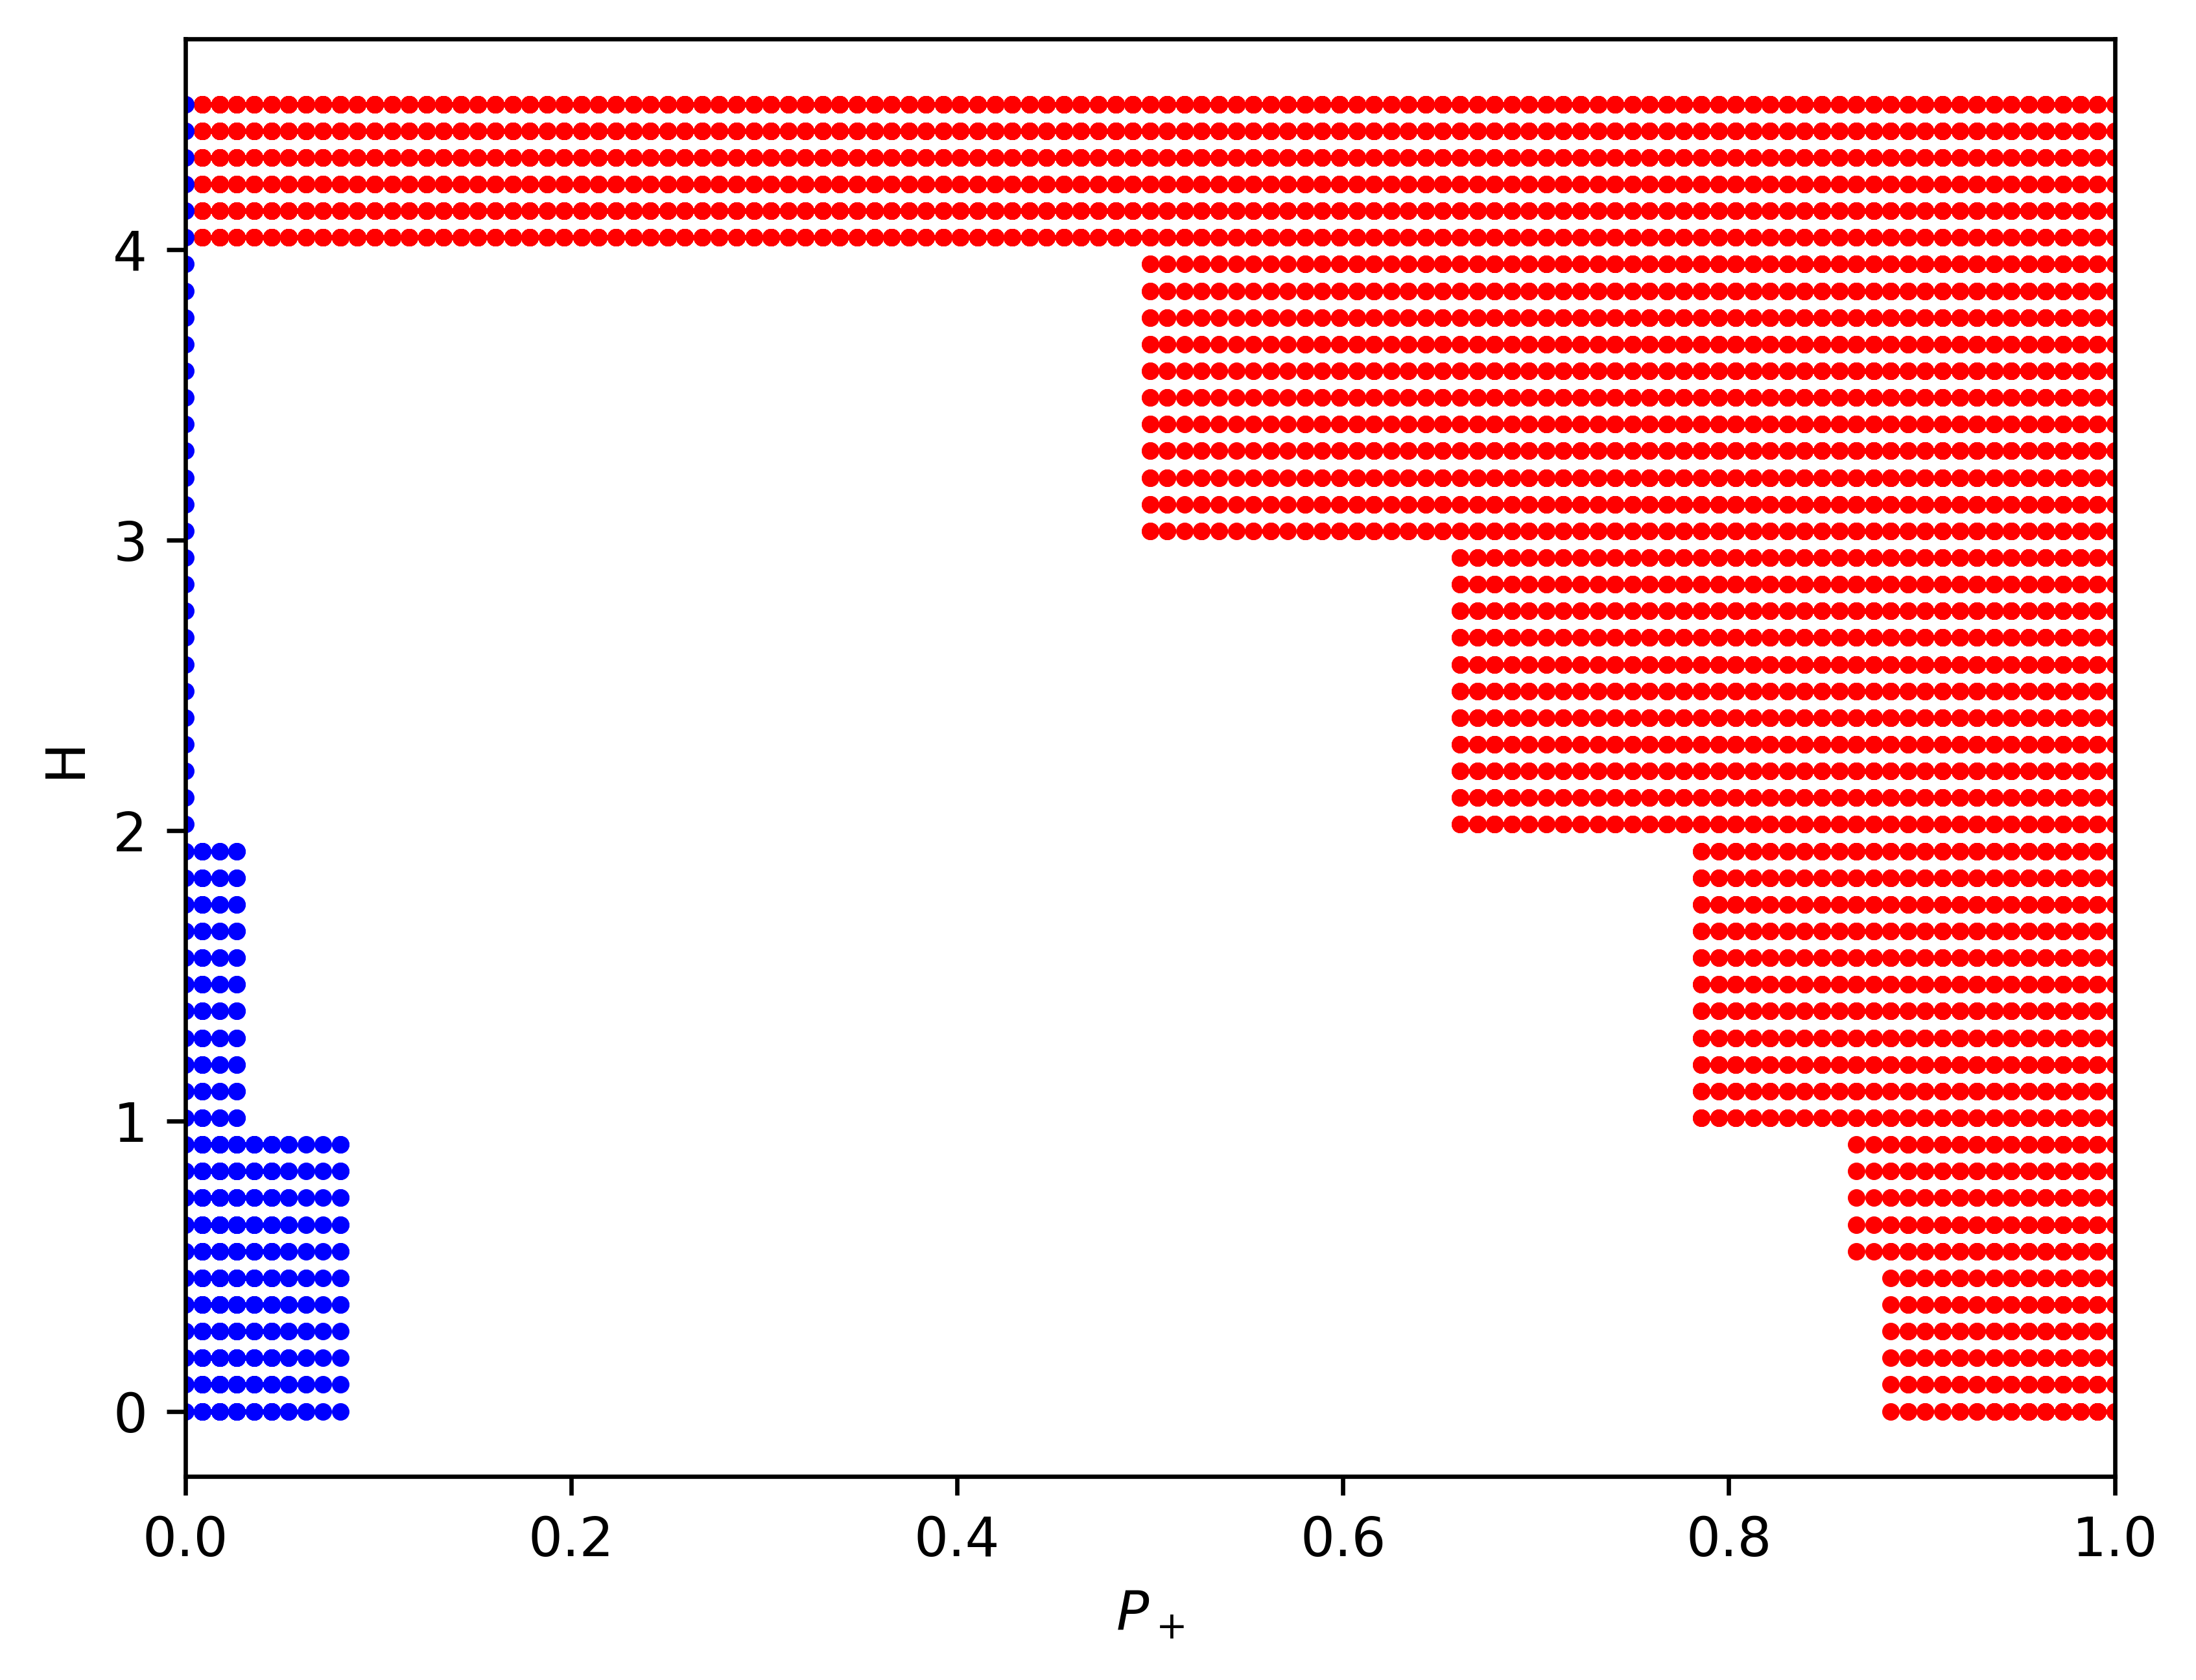
\includegraphics[width=0.8\textwidth]{images/P+_afm_fm(H)_filled.png}
		\caption{Phase diagram at $T = 0$ in an external magnetic field. Blue dots represent the antiferromagnetic state; red dots represent the ferromagnetic state.}
		\label{fig:P+_afm_fm(H)}
	\end{figure}
	
	An external magnetic field shifts the state boundaries. For $h/J > 1$, a spin-flop transition occurs at $P_+ < 0.1$ in some cases, and for $h/J > 2$, it occurs in all. A spin glass exists at $P_+ = 0.5$ for $h/J < 3$, as no sample satisfies the definition of either a ferromagnet (Equation \eqref{eq:ferr_deffinition}) or an antiferromagnet (Equation \eqref{eq:aferr_deffinition}). For $h/J > 4$, all samples transition to a ferromagnetic state. 
	
	The staircase-like behavior on the diagram can be explained by the competition between internal interaction energy and Zeeman energy. At critical field values, the Zeeman energy dominates, causing phase transitions across groups of samples with varying $P_+$.
	
	It should be noted that open boundary conditions may introduce significant influence on results. For example, a cases with $P_+ = 0.2$ (Figures \ref{fig:Mgs(P+)} and \ref{fig:P_AFM_FM_Mmax}) exhibits antiferromagnetic properties due to ferromagnetic bonds ($J_{ij} = 1$) being concentrated along the edges.
	
	\section{Conclusion}
	
	An exact solution for the ground state of the Edwards-Anderson model on a simple square lattice of $8 \times 8$ spins has been obtained and analyzed using an complete enumeration method. The developed algorithm enables the calculation of degeneracy, energy, and spin excess for each of the $2^N$ possible states, facilitating studies at zero temperature and in the presence of a nonzero external magnetic field $h/J$.
	
	It has been demonstrated that the macroscopic degeneracy of the ground state in finite-sized frustrated spin systems within the Edwards-Anderson model is governed by the combinatorics of frustration in  Type-II plaquettes, i.e., by the number of ways to arrange frustrated spin pairs on the lattice. An algorithm has been proposed for calculating energy, spin excess, and ground state configurations based on the determination of frustration locations.
	
	It was established that Type-II plaquettes are the sole source of frustration in the ground state in the absence of an external magnetic field. In energy-minimizing configurations, frustrations may also appear between Type-II plaquettes or between a frustrated plaquette and the lattice boundary, depending on the distances and boundary conditions. Macroscopic ground state degeneration implies alternative arrangements of frustrations.
	
	The dependence of the ground state spin excess in the Edwards-Anderson model on the external magnetic field at $T \to 0$ exhibits a discrete (stepped, staircase-like) character. This behavior is caused by the discrete structure of the density of states. Critical values of the external magnetic field, where giant peaks in residual entropy are observed, have been calculated. The nature of these entropy peaks arises from the fact that at certain critical field values, multiple spin configurations with different interaction and Zeeman energies—but the same total energy—contribute equally to the ground state. Degeneracies of states with identical total energy are summed.
	
	The phase diagram $h - P_+$ at $T = 0$ is obtained. The exact solution allowed us to establish the conditions for the existence of low-temperature states depending on the external magnetic field and the concentration of exchange bonds $P_+$. The maximum absolute value of spin excess of the ground state is a general criterion that allows us to establish the existence of low-temperature states: antiferromagnetic, spin-glass, and ferromagnetic. The application of an external magnetic field leads to a shift of phases. The stepwise behavior of the diagram is explained by the competition of exchange interaction energy and Zeiman energy
	
	The problem of determining the maximum possible quantity of frustrations as a function of the number of spins in a system, for a given lattice type in the Ising model with both antiferromagnetic and ferromagnetic exchange interactions, is of interest, as the presence of frustrations gives rise to new properties.
	It has been shown that in the Edwards-Anderson model, systems with twofold ground state degeneracy can exist, and configurations of minimum energy may include frustrations. Additionally, the placement of frustrations in ground state configurations (i.e., the degeneracy of states with nonzero spin excess) and the suppression of frustrations by an external magnetic field could be subjects of further research.
	
	In the spin glass there is no order in the arrangement of Type-II plaquettes.
	Type-II plaquettes are a source of frustrations.
	In contrast to spin glass, highly frustrated spin system has a dense packing or ordering of Type-II plaquettes.  
	The degeneracy depends on the number of Type-II plaquettes and their mutual arrangement.
	Frustrated bonds can not only change their localization on the lattice in degenerate ground state configurations but also alter the relative number of ferromagnetic and antiferromagnetic bonds.  
	Therefore, macroscopically degenerate ground state configurations of spin glass and highly frustrated spin system may have different spin excess.
	
	It would be interesting to explore the problem of Type-II plaquettes in the highly frustrated spin system model on a three-dimensional pyrochlore lattice.
	
	\section{Acknowledgments}
	
	The research was supported by the Russian Science Foundation grant No. 24-71-10069, https://rscf.ru/en/project/24-71-10069/.
	
	\bibliography{mybibfile}
	
	
\end{document}